\documentclass[]{usiinfthesis}
\usepackage{lipsum}
\usepackage[draft]{fixme}
%\usepackage{setspace}
%\setstretch{1.05}

\usepackage[svgnames,table]{xcolor}
\usepackage{tikz}
\usepackage{cleveref}
\usepackage{mdframed}
\usepackage{listings}
\usepackage{inconsolata}
\usepackage{paralist}
\usepackage{enumitem}
\usepackage{tabularx}
\usepackage{pifont}
\usepackage{multirow}
\usepackage{multicol}
\usepackage{wrapfig}

\newcommand{\cmark}{\ding{51}}%
\newcommand{\xmark}{\ding{55}}%

\newcommand{\USI}{Universit\`a della Svizzera Italiana}

\usetikzlibrary{automata}
\usetikzlibrary{shapes,arrows}


\newcommand{\hlbox}[3]{
\begin{mdframed}[backgroundcolor=#2!00]
\rightline{ \footnotesize \emph{MRQ} }
% \ 

\centering
#1
\end{mdframed}
}

\newcommand{\discuss}[1]{\todo[color=yellow]{\textbf{[DISCUSS]} #1}}
% \newcommand{\done}[1]{\todo[color=cyan]{\footnotesize \textbf{[DONE]} #1}}
\newcommand{\done}[1]{}

\newcommand{\rquestion}[1]{\hlbox{#1}{yellow}{Research Question}}

\newcommand{\eg}{\textit{e.g.}}
\newcommand{\ie}{\textit{i.e.}}
\newcommand{\etc}{\textit{etc.}}
\newcommand{\adhoc}{\textit{ad-hoc}}
\newcommand{\perse}{\textit{per se}}
\newcommand{\circa}{\textit{circa}}

\newcommand{\phd}{Ph.D.}

\newcommand{\code}[1]{\texttt{#1}}
\newcommand{\lang}[1]{\textsc{#1}}
\newcommand{\host}[1]{\textsl{#1}}

\newcommand{\api}{API}

\newcommand{\java}{\lang{Java}}
\newcommand{\csharp}{\lang{C\#}}
\newcommand{\cc}{\lang{C}}
\newcommand{\cpp}{\lang{C++}}
\newcommand{\smalltalk}{\lang{Smalltalk}}
\newcommand{\javascript}{\lang{JavaScript}}
\newcommand{\haskell}{\lang{Haskell}}
\newcommand{\scala}{\lang{Scala}}
\newcommand{\clojure}{\lang{Clojure}}
\newcommand{\ql}{\lang{QL}}
\newcommand{\fortran}{\lang{Fortran}}
\newcommand{\cobol}{\lang{Cobol}}
\newcommand{\pascal}{\lang{Pascal}}
\newcommand{\apl}{\lang{APL}}
\newcommand{\basic}{\lang{Basic}}
\newcommand{\swift}{\lang{Swift}}
\newcommand{\php}{\lang{PHP}}
\newcommand{\racket}{\lang{Racket}}
\newcommand{\rust}{\lang{Rust}}
\newcommand{\kotlin}{\lang{Kotlin}}
\newcommand{\ml}{\lang{ML}}

\newcommand{\jvm}{JVM}
\newcommand{\jvmti}{JVMTI}
\newcommand{\jni}{JNI}
\newcommand{\lilith}{Lilith}

\newcommand{\instanceof}{\code{instanceof}}
\newcommand{\throw}{\code{throw}}
\newcommand{\smu}{\code{sun.misc.Unsafe}}
\newcommand{\cce}{\code{ClassCastException}}
\newcommand{\npe}{\code{NullPointerException}}
\newcommand{\setjmp}{\code{setjmp}}
\newcommand{\longjmp}{\code{longjmp}}

\newcommand{\asm}{ASM}
\newcommand{\jnif}{JNIF}

\newcommand{\eval}{\code{eval}}

\newcommand{\github}{\host{GitHub}}
\newcommand{\gitlab}{\host{GitLab}}
\newcommand{\bitbucket}{\host{Bitbucket}}
\newcommand{\sourceforge}{\host{SourceForge}}
\newcommand{\maven}{\host{Maven}}
\newcommand{\mavencentral}{\host{Maven Central}}
\newcommand{\npm}{\host{npm}}
\newcommand{\boa}{\host{Boa}}
\newcommand{\candoia}{\host{Candoia}}
\newcommand{\lgtm}{\host{lgtm}}
\newcommand{\rascal}{\host{Rascal}}
\newcommand{\sourcegraph}{\host{sourcegraph}}
\newcommand{\bitly}{\host{Bitly}}

\newcommand{\hdr}{\rowcolor{header-color}}
\newcommand{\alt}{\rowcolor{alt-row-color}}
\newcommand{\row}{}

\newcommand{\unsafe}{\emph{Unsafe}}

\definecolor{header-color}{HTML}{D1D1D1}
\definecolor{alt-row-color}{HTML}{ECECEC}

\newcommand{\artstyle}[1]{\textsl{#1}}
\newcommand{\artexp}[2]{\artstyle{#1}:\artstyle{#2}}
\newcommand{\art}[3]{\artstyle{#1}:\artstyle{#2}\footnote{\url{#3}}}

\newcommand{\member}[1]{\emph{#1}}
\newcommand{\smugroup}[1]{\textsl{#1}}
\newcommand{\stackoverflow}{Stack Overflow}



\definecolor{lightgray}{rgb}{0.98,0.98,0.98}
\definecolor{lightblue}{rgb}{0.85,0.95,1}
\definecolor{gray}{rgb}{0.2,0.2,0.2}

% \definecolor{light-orange}{rgb}{1,0.6,0}

\definecolor{diffstart}{named}{Grey}
\definecolor{diffincl}{named}{Green}
\definecolor{diffrem}{named}{OrangeRed}
\definecolor{hl}{named}{OrangeRed}

\setminted[java]{
	baselinestretch=1,
	bgcolor=lightgray,
	fontsize=\footnotesize,
	highlightcolor=lightblue,
	tabsize=4,
	linenos
}

\setminted[scala]{
	baselinestretch=1,
	bgcolor=lightgray,
	fontsize=\footnotesize,
	highlightcolor=lightblue,
	tabsize=4,
	linenos
}

\lstdefinestyle{java}{
	language=java,
	tabsize=4,
	basicstyle=\scriptsize\ttfamily,
	numbers=left,
	numberstyle=\tiny\color{gray},
	numbersep=4pt,
	xleftmargin=0.2cm,
	% mathescape=true,
	keywordstyle=\color{blue}\textbf,
	stringstyle=\textcolor{magenta},
	captionpos=b,
	emph={Object, String, Integer, System, ClassCastException, Foo},
	emphstyle={\color{lightblue}},
    morecomment=[f][\color{diffstart}]{@@},
    morecomment=[f][\color{diffincl}]{+\ },
	morecomment=[f][\color{diffrem}]{-\ },
}

\lstdefinestyle{ql}{
	language=sql,
	tabsize=2,
	basicstyle=\scriptsize\ttfamily,
	numbers=left,
	numberstyle=\tiny\color{gray},
	numbersep=4pt,
	xleftmargin=0.2cm,
	mathescape=true,
	keywordstyle=\color{blue}\textbf,
	stringstyle=\color{magenta},
	captionpos=b,
	showstringspaces=false,
	keywords=[2]{import, predicate, java, instanceof},
	emph={CastExpr, PrimitiveType},
	emphstyle={\color{lightblue}}
}

\lstdefinestyle{bytecode}{
	language=java,
	tabsize=4,
	basicstyle=\footnotesize\ttfamily,
	numbers=left,
	numberstyle=\tiny\color{gray},
	numbersep=4pt,
	xleftmargin=0.2cm,
	% mathescape=true,
	keywordstyle=\color{blue}\textbf,
	stringstyle=\textcolor{magenta},
	captionpos=b,
	emph={ldc,invokestatic,astore_1,aload_1,invokevirtual,checkcast,astore_2},
	emphstyle={\color{lightblue}},
    morecomment=[f][\color{diffstart}]{@@},
    morecomment=[f][\color{diffincl}]{+\ },
	morecomment=[f][\color{diffrem}]{-\ },
}


% DONE: Changed "why" question.
\newcommand{\urqA}{To what extent does the Unsafe API impact common application code?}
\newcommand{\urqB}{How and when are Unsafe features used?}

% DONE: Is casting used in common application code? Yes. Change question.
% \todo{To what extent is}
% CRQ2: How and \underline{why} casts are used?
\newcommand{\crqA}{How frequently is casting used in common application code?}
\newcommand{\crqB}{How and when casts are used?}
\newcommand{\crqC}{How recurrent are the patterns for which casts are used?}
\newcommand{\nproject}{24}
\newcommand{\nloc}{1,439,913}
\newcommand{\nexpr}{4,324,652}
\newcommand{\ncast}{8,627}
\newcommand{\nmethod}{121,665}
\newcommand{\nmethodwithcast}{6,091}
\newcommand{\neqm}{669}
\newcommand{\castratio}{3.92\%}



%change 'sl' to 'bf' for bold, or 'normalfont' for no special
%formatting
\captionsetup{labelfont={sl,sf}}

\lstdefinelanguage{algebra}
{morekeywords={import,sort,constructors,observers,transformers,axioms,if,
else,end},
sensitive=false,
morecomment=[l]{//s},
}

\title{When and How \lang{Java} Developers Give Up Static Type Safety} %compulsory
\subtitle{Subtitle: Reinventing the World} %optional 
\author{Luis Mastrangelo} %compulsory
\advisor{Prof. Matthias Hauswirth} %compulsory
\coadvisor{Prof. Nathaniel Nystrom} %optional
\Day{First} %compulsory
\Month{March} %compulsory
\Year{2019} %compulsory, put only the year
\place{Lugano} %compulsory
% Not used: Both Ph.D. Program Directors hard-coded in the class file.
\programDirector{Prof. Walter Binder \& Prof. Olaf Schenk} %compulsory

\committee{%
  \committeeMember{Prof. Antonio Carzaniga}{\USI, Switzerland}
  \committeeMember{Prof. Gabriele Bavota}{\USI, Switzerland}
  \committeeMember{Prof. Jan Vitek}{Northeastern University \& Czech Technical University}
  \committeeMember{Prof. Hridesh Rajan}{Iowa State University}
  %there can as many members as you like
} %the committee is compulsory

\dedication{To my beloved} %optional
\openepigraph{Someone said \dots}{Someone} %optional

\makeindex %optional, also comment out \theindex at the end

\begin{document}

\maketitle %generates the titlepage, this is FIXED

\frontmatter %generates the frontmatter, this is FIXED


% DONE: Reverse the argument, we want to help, and this is how.
\begin{abstract}
The main goal of a static type system is to prevent certain kind of errors from happening at run-time.
A type system is formulated as a set of constraints that gives any expression or term in a program a well-defined type.
Yet
% DONE: "they" means all type systems, need to be more precise
% they
mainstream programming languages are endowed with type systems that
provide the means to circumvent their constraints through the \emph{unsafe intrinsics} and \emph{casting} mechanisms.

We want to understand how and when developers circumvent these constraints.
This knowledge can be:
\begin{inparaenum}[a)]
% DONE: Make a) a noun, "a ..."
% \item useful to make informed decisions for current and
% future language designers,
\item a recommendation for current and future language designers
to make informed decisions
\item a reference for tool builders, \eg{},
by providing more precise or new refactoring analyses,
\item a guide for researchers to test new language features,
or to carry out controlled programming experiments, and
\item a guide for developers for better practices.
\end{inparaenum}

We plan to empirically study how these two mechanisms
--- unsafe intrinsics and casting ---
are used by \java{} developers to circumvent the static type system.
% Our study focus on how these features are used in \lang{Java}.
% given its wide usage and relevance for both research and industry.
We have devised (%
% for the \java{}'s Unsafe \api{}
for a subset of unsafe intrinsics%
) and
% DONE: Make continuous
we are devising (for casting)
% DONE: Explain what "usage patterns" are
usage patterns,
recurrent programming idioms to solve a specific issue.
We believe that having usage patterns can help us to better categorize use cases and
thus understand how those features are used.

% These patterns can provide an insight on how the language is being used by developers in real-world applications.
\end{abstract}

% item useful to make informed decisions for current \& future language designers, not only \java{},

% Programming languages offer a wide range of features that aim to improve programmers productivity.
% However, to better drive the future evolution of any programming language,
% we believe it is AVOID:paramount to have a thorough understanding of how these features are actually being used in real codebases.

% Understanding how developers make use of language features can be helpful to a AVOID:broad audience besides language designers.
% It can aid tool builders to make more realistic assumptions;
% researchers to improve the state-of-the-art;
% and developers to implement more efficient and effective solutions by providing them best practices.

% In this proposal, we target two specific features, namely, casting and the unsafe API.
% \java{} features, namely, \emph{casting}, \emph{reflection}, \emph{exception handling} and the \emph{unsafe} \api{}.
% We give the rationale behind our decision on why we chose these features.
% We plan to devise language and API usage patterns at large-scale to properly assess this broad audience.
% We hope that having a better understanding on how these features are used, we can make informed decisions for these driving forces.


\begin{abstract}[Zusammenfassung]
optional, use only if your external advisor requires it in his/er
language 
\\

\lipsum
\end{abstract}

\begin{acknowledgements}
\lipsum 
\end{acknowledgements}

\tableofcontents 
\listoffigures %optional
\listoftables %optional

\mainmatter

\chapter{Introduction}
\lipsum[1-4]
\section{Let's start!}

\lipsum



\chapter[Short title]{A chapter title which will run over two lines --- it's for
  testing purpose}

\lipsum[1-2]

\section{The first \textsc{Section}}

Here is some text with \textsc{SmallCaps} in normal font.

\lipsum[3-4]

 \section{The second, math section}
\begin{center}
  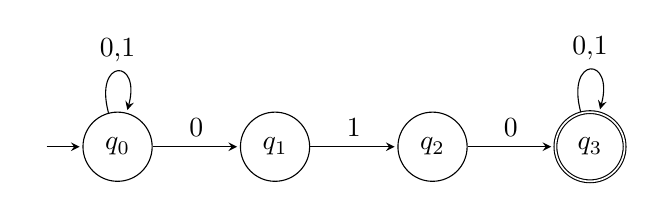
\begin{tikzpicture}[shorten >=1pt,node distance=2cm,auto, initial text=, >=stealth] 
    \node[state, initial] (q0) {$q_0$};
    \node[state] (q1) [right of=q0] {$q_1$};
    \node[state] (q2) [right of=q1] {$q_2$};
    \node[state, accepting] (q3) [right of=q2] {$q_3$};
    \path[->]
    (q0) 
    edge [loop above] node {0,1} ()
    edge  node {0} (q1)
    (q1)
    edge  node {1} (q2)
    (q2)
    edge node {0} (q3)
    (q3)
    edge [loop above] node {0,1} ()
;
  \end{tikzpicture}
\end{center}

\textbf{Theorem 1 (Residue Theorem).}
Let $f$ be analytic in the region $G$ except for the isolated singularities $a_1,a_2,\ldots,a_m$. If $\gamma$ is a closed rectifiable curve in $G$ which does not pass through any of the points $a_k$ and if $\gamma\approx 0$ in $G$ then
\[
\frac{1}{2\pi i}\int_\gamma f = \sum_{k=1}^m n(\gamma;a_k) \text{Res}(f;a_k).
\]
\textbf{Theorem 2 (Maximum Modulus).}
\emph{Let $G$ be a bounded open set in $\mathbb{C}$ and suppose that $f$ is a continuous function on $G^-$ which is analytic in $G$. Then}
\[
\max\{|f(z)|:z\in G^-\}=\max \{|f(z)|:z\in \partial G \}.
\]

\section[third]{A very very long section, titled ``The third section'', with
  a rather  short text alternative (third)}
\lipsum \texttt{Some Test}
\lstset{language=algebra,linewidth=0.95\linewidth,breaklines=true,numbers=left,
basicstyle=\ttfamily,numberstyle=\tiny,escapeinside={//*}{\^^M},
mathescape=true}
\begin{lstlisting}
import IntSpec, ItemSpec;

sort cart; //*\label{sort}

constructors //*\label{begin-sig}
create() $\longrightarrow$ cart;
insert(cart, item) $\longrightarrow$ cart;
observers
amount(cart) $\longrightarrow$ int;
transformers
delete(cart, item) $\longrightarrow$ cart; //*\label{end-sig}

axioms //*\label{begin-axioms}
forall c: cart, i, j: item 

amount(create()) $=$ 0; //*\label{begin-amount}
amount(insert(c,i)) $=$ amount(c) $+$ price(i); //*\label{end-amount}
delete(create(),i) $=$ create(); //*\label{begin-delete}
delete(insert(c,i),j) $=$
if (i =$\:$= j) c
else insert(delete(c,j),i); //*\label{end-axioms}
end
\end{lstlisting}

As you can easily see from the above listing \citet{bbggs:iet07}
define something weird based on the BPEL specification
\citep{bpelspec}.

% shows all citations. Nope.
% \nocite{*}

\chapter{Introduction}

In programming language design, the main goal of a \emph{static} type system is to prevent certain kind of errors from happening at run-time.
A type system is formulated as a set of constraints that gives any expression or term in a program a well-defined type.
As~\cite{pierceTypesProgrammingLanguages2002} states:
``A type system can be regarded as calculating a kind of \emph{static} approximation to the run-time behaviors of the terms in a program.''
These constraints are enforced by the \emph{type-checker} either when compiling or linking the program.
Thus, any program not satisfying the constraints stated within a type system is simply rejected by the type-checker.

Nevertheless, often the static approximation provided by a type system is not precise enough.
Being static, the analysis done by the type-checker needs to be conservative:
It is better to reject programs that are valid,
but whose validity cannot be ensured by the type-checker,
rather than accept some invalid programs.
However, there are situations when the developer has more information
about the program that is too complex to explain in terms of typing constraints.
To that end, programming languages often provide \emph{mechanisms} that 
make the typing constraints less strict
to permit more programs to be valid,
at the expense of causing more errors at run-time.
These mechanisms are essentially two:
\emph{Unsafe Intrinsics} and \emph{Casting}.

\textbf{Unsafe Intrinsics.}
Unsafe intrinsics is the ability to perform certain operations \emph{without} being checked by the compiler.
They are \emph{unsafe} because any misuse made by the programmer can compromise the entire system, \eg{},
corrupting data structures without notice, or
crashing the run-time system.
Unsafe intrinsics can be seen in safe languages, \eg{},
\lang{Java},
\lang{C\#},
\lang{Rust}, or
\lang{Haskell}.
Foreign Function Interface (\emph{FFI}), \ie{}, calling native code from within a safe environment is unsafe.
It is so because the run-time system cannot guarantee anything about the native code.
In addition to FFI, some safe languages offer so-called \emph{unsafe} blocks, \ie{}, making unsafe operations within the language itself, \eg{},
\lang{C\#}%
\urlnote{https://docs.microsoft.com/en-us/dotnet/csharp/language-reference/language-specification/unsafe-code}
and
\lang{Rust}.%
\urlnote{https://doc.rust-lang.org/book/second-edition/ch19-01-unsafe-rust.html}
Other languages provide an API to perform unsafe operations, \eg{},
\lang{Haskell}\footnote{\url{http://hackage.haskell.org/package/base-4.11.1.0/docs/System-IO-Unsafe.html}}
and
\lang{Java}.
But in the case of \lang{Java}, the API to make unsafe operations,
\code{sun.misc.Unsafe},
is unsupported\footnote{\url{http://www.oracle.com/technetwork/java/faq-sun-packages-142232.html}}
and undocumented.
It was originally intended for internal use within the JDK, but as we shall see later on, it is used outside the JDK as well.

\textbf{Casting.}
Programming languages with subtyping such as \java{} or \cpp{} provide a mechanism to \emph{view} an expression as a different type as it was defined.
This mechanism is often called \emph{casting} and takes the form \code{(T) t}.
Casting can be in two directions: \emph{upcast} and \emph{downcast}.
An upcast conversion happens when converting from a reference type $S$ to a reference type $T$, provided that $T$ is a \emph{supertype} of $S$.
An upcast does not require any explicit casting operation nor compiler check.
However, as we shall see later on, there are situations where an upcast requires an explicit casting operation.
On the other hand, a downcast happens when converting from a reference type $S$ to a reference type $T$, provided that $T$ is a \emph{subtype} of $S$.
Unlike upcasts, downcasts require a run-time check to verify that the conversion is indeed valid.
This implies that downcasts provide the means to bypass the static type system.
By avoiding the type system, downcasts can pose potential threats, because it is like the developer saying to the compiler: \emph{``Trust me here, I know what I'm doing''}.
Being a escape-hatch to the type system,
a cast is often seen as a design flaw or code smell~\citep{tufanoWhenWhyYour2015} in an object-oriented system.


\section{Research Question}

If static type systems aim to prevent certain kind of errors from happening at run-time,
yet they provide the means to circumvent their constraints,
why exactly does one need to do so?
Are these mechanisms actually used in real-world code?
If yes, then how so?
This triggers our \textbf{main research question}:

\begin{mdframed}
\rightline{\footnotesize \emph{MRQ}}

\centering
For what purpose do developers circumvent static type systems?
\end{mdframed}

We have confidence that this knowledge can be:
\begin{inparaenum}[a)]
\item a reference for current and future language designers
to make informed decisions about programming languages,
\eg{}, the adoption of \emph{Variable Handles} in \java{} 9~\citep{jep193},
or the addition of \emph{Smart Casts} in \lang{Kotlin},\footnote{\url{https://kotlinlang.org/docs/reference/typecasts.html\#smart-casts}}
\item a reference for tool builders, \eg{}, by providing more precise or new refactoring analyses,
\item a guide for researchers to test new language features, \eg{}, \cite{wintherGuardedTypePromotion2011} or to carry out controlled experiments about programming, \eg{}, \cite{stuchlikStaticVsDynamic2011} and
\item a guide for developers for best or better practices.
\end{inparaenum}

To answer our question above,
we empirically studied how the two aforementioned mechanisms---unsafe intrinsics and casting---are used by developers.
Since any kind of language study must be language-specific,
we focus on \java{} given its wide usage and relevance for both
research and industry.%
\footnote{\url{https://www.tiobe.com/tiobe-index/}}
Moreover, we focus on the \java{} Unsafe API to study unsafe intrinsics,
given than the Java Native Interface already has been studied
in~\cite{tanSafeJavaNative2006,tanEmpiricalSecurityStudy2008,kondohFindingBugsJava2008,sunNativeGuardProtectingAndroid2014,liFindingBugsExceptional2009}.
Similarly, although casting uses run-time type information like
the \java's reflection \api{},
the reflection \api{} has been studied in
\cite{livshitsImprovingSoftwareSecurity2006,livshitsReflectionAnalysisJava2005,landmanChallengesStaticAnalysis2017}.

To better drive our \emph{main research question},
we propose to answer the following set of sub-questions.
To answer these research sub-questions,
we have devised \emph{usage patterns} for both the Unsafe \api{} and casting.
Usage patterns are \emph{recurrent programming idioms} used by developers to solve a specific issue.
We believe that having usage patterns can help us to better categorize use cases and
thus understand how these mechanisms are used.
These patterns can provide an insight into how the language is being used by developers in real-world applications.
Overall these sub-questions will help us to answer our MRQ:

\subsection*{Unsafe API}

\begin{enumerate}[label=$RQ/U\arabic*:$,leftmargin=3.4\parindent]
\item {\bf \urqA} \urqAdesc{}
\item {\bf \urqB} \urqBdesc{}
\end{enumerate}

These questions have been already answered in our previous published
study on the Unsafe API in \java{}~\citep{mastrangeloUseYourOwn2015}.

\subsection*{Casting}

\begin{enumerate}[label=$RQ/C\arabic*:$,leftmargin=3.4\parindent]
\item {\bf \crqA} \crqAdesc{}
\item {\bf \crqB} \crqBdesc{}
\item {\bf \crqC} \crqCdesc{}
\end{enumerate}

The results of this study have been submitted for publication to \conf{OOPSLA}{19}.

\section{Thesis Outline}

The rest of this thesis is as follows.
In Chapter~\ref{cha:literature-review} we give a review of the literature in empirical studies of programming languages features.
In particular, Sections~\ref{sec:literature-review:unsafe} and~\ref{sec:literature-review:casting} review the \emph{state-of-the-art} of the different aspects related to the two proposed studies.
Chapter~\ref{cha:unsafe} presents a summary of our \unsafe{} study;
while in Chapter \ref{cha:casts} we present our \emph{casting} study.
Finally, Chapter~\ref{cha:conclusions} presents the conclusions for the thesis.

The Appendix~\ref{ap:ql} contains an introduction to \ql{}%
---the language we used to approximate automatic detection of patterns---%
and reference material used in our casting study.
Appendix~\ref{ap:jnif}---although not directly related---%
describes our bytecode analysis library used in some experiments in both Chapters~\ref{cha:unsafe} and~\ref{cha:casts}.

\chapter{Literature Review}
\label{cha:literature-review}

Understanding how developers use language features
and \api{}s is a broad topic.
There is plenty of research in the computer science literature about
empirical studies of programs which involves multiple \emph{dimensions}
directly related to our plan.
Over the last decades,
researchers always have been interested in understanding what
kind of programs developers write.
% The motivation behind these studies is quite broad,
% and has been shifted to the needs of researchers,
% together with the evolution of computer science itself.

% For instance, to measure the advantages between compilation and interpretation in \basic{},
% \cite{hammondBASICEvaluationProcessing1977} studied a representative dataset of programs.
% \cite{knuthEmpiricalStudyFORTRAN1971} started to study \fortran{} programs.
% By knowing what kind of programs arise in practice,
% a compiler optimizer can focus in those cases,
% and therefore can be more effective.
% Adding to Knuth's work,%
% ~\cite{shenEmpiricalStudyFortran1990} conducted an empirical study for
% parallelizing compilers.
% Similar works have been done for
% \cobol{}~\cite{salvadoriStaticProfileCOBOL1975,chevanceStaticProfileDynamic1978},
% \pascal{}~\cite{cookContextualAnalysisPascal1982},
% and \apl{}~\cite{saalPropertiesAPLPrograms1975,saalEmpiricalStudyAPL1977} programs.
% \cite{millerEmpiricalStudyReliability1990,millerFuzzRevisitedReexamination1995,forresterEmpiricalStudyRobustness2000}
% studied the reliability of programs using \emph{fuzz} testing.
% \cite{dieckmannStudyAllocationBehavior1999} studied the memory allocating
% behavior in the SPECjvm98 benchmarks.%
% \footnote{\url{https://www.spec.org/jvm98/}}

% But there is more than empirical studies at the source code level.
% A machine instruction set is effectively another kind of language.
% Therefore, its design can be affected by how compilers generate machine code.
% Several studies targeted the \jvm{}~\cite{collbergEmpiricalStudyJava2007,odonoghueBigramAnalysisJava2002,antonioliAnalysisJavaClass1998};
% while~\cite{cookEmpiricalAnalysisLilith1989} did a similar study for \lilith{} in the past.

The importance of conducting empirical studies of programs gave rise to the International Conference on Mining Software Repositories%
\footnote{\url{http://www.msrconf.org/}}
in 2004.

\section*{Outline}

When conducting empirical studies about programs,
multiple dimensions are involved.
The first one is \emph{What to analyse?}
Benchmarks and corpora are used as a source of programs to analyse.
Another aspect is how to select good candidate projects from a large-base software repository.
This is presented in Section~\ref{sec:literature-review:benchmarks}.
After the selection of programs to analyse is set,
comes the question \emph{how to analyse them?}
An overview of what tools are available to extract information from software repositories is given in Section~\ref{sec:literature-review:mining}.
With this infrastructure, \emph{what questions do researchers ask?}
In Section~\ref{sec:literature-review:largescale},
we give an overview of large-scale empirical studies that show what kind of questions researchers ask.
In particular, this section ends by presenting the related work more specific to the Unsafe API and Casting in Sections~\ref{sec:literature-review:unsafe} and \ref{sec:literature-review:casting} respectively.
Finally, Section~\ref{sec:literature-review:conclusions} concludes this chapter.

\section{Benchmarks and Corpora}
\label{sec:literature-review:benchmarks}

Benchmarks are crucial to properly evaluate and measure product development.
This is key for both research and industry.
One popular benchmark suite for \java{} is the DaCapo Benchmark~\citep{blackburnDaCapoBenchmarksJava2006}.
This suite has been already cited in more than thousand publications, showing how important is to have reliable benchmark suites.
The SPECjvm2008\footnote{\url{https://www.spec.org/jvm2008/}}
(Java Virtual Machine Benchmark)
and
SPECjbb2000\footnote{\url{https://www.spec.org/jbb2000/}}
(Java Business Benchmark)
are another popular \java{} benchmark suite.

Another suite has been developed by~\cite{temperoQualitasCorpusCurated2010}.
They provide the Qualitas Corpus, a corpus of curated open source systems to facilitate empirical studies on source code.
On top of the Qualitas Corpus,~\cite{dietrichXCorpusExecutableCorpus2017} provide an executable corpus of \java{} programs.
This allows any researcher to experiment with both static and dynamic analysis.

For any benchmark or corpus to be useful and reliable,
it must faithfully represent real-world code.
For instance,
DaCapo applications were selected to be diverse real applications and
ease of use, but they ``excluded GUI applications since they are difficult
to benchmark systematically.''
Along these lines, \cite{allamanisMiningSourceCode2013} go one step further and provide a large-scale (14,807) curated corpus of open source \java{} projects.

With the advent of cloud computing,
several source code management (SCM) hosting services have emerged, \eg{},
\github{}, \gitlab{}, \bitbucket{}, and \sourceforge{}.
These services allow the developer to work with different SCMs, \eg,
Git, Mercurial, Subversion to host their open source projects.
These projects are usually taken as a representation of
real-world applications.
Thus, while not curated corpora, these hosting services are
commonly used to conduct empirical studies.

Another dimension to consider when analysing large codebases, is how relevant the repositories are.
\cite{lopesDeJaVuMapCode2017} conducted a study to measure code duplication in \github{}.
They found out that much of the code there is actually duplicated.
This raises a flag when considering which projects to analyse when mining software repositories.

\cite{baxterCloneDetectionUsing1998} propose a clone detection algorithm using Abstract Syntax Trees,
while \cite{riegerVisualDetectionDuplicated} propose a visual detection for clones.
\cite{yuanCMCDCountMatrix2011,chenReplicationReproductionCode} instead propose Count Matrix-based approach to detect code clones.

\cite{nagappanDiversitySoftwareEngineering2013} have developed the Software Projects Sampling (SPS) tool.
SPS tries to find a maximal set of projects based on representativeness and diversity.
Diversity dimensions considered include total lines of code,
project age, activity, number of contributors, total code churn,
and number of commits.

\section{Tools for Mining Software Repositories}
\label{sec:literature-review:mining}

When talking about mining software repositories,
we refer to extracting any kind of information from large-scale codebase repositories. 
Usually doing so requires several engineering but challenging tasks.
The most common being downloading, storing, parsing, analysing and
properly extracting information from different kinds of artifacts.
In this scenario, there are several tools that allows a researcher or developer to query information about software repositories.

%\urlnote{https://wiki.openjdk.java.net/display/Compiler/Java+Corpus+Tools}
\cite{urmaProgrammingLanguageEvolution2012} evaluated seven source code
query languages:
\emph{Java Tools Language}~\citep{cohenJTLJavaTools},
\emph{SOUL}~\citep{derooverSOULToolSuite2011},
\emph{Browse-By-Query}\footnote{\url{http://browsebyquery.sourceforge.net/}},
\emph{JQuery}~\citep{volderJqueryGenericCode2006},
\emph{.QL}~\citep{moorKeynoteAddressQL2007},
\emph{Jackpot}\footnote{\url{http://wiki.netbeans.org/Jackpot}}, and
\emph{PMD}\footnote{\url{https://pmd.github.io/}}.
They have implemented, whenever possible,
four use cases using the tools mentioned above.
They concluded that only \emph{SOUL} and \emph{.QL} have the minimal features to implement all their use cases.

\cite{dyerBoaLanguageInfrastructure2013,dyerDeclarativeVisitorsEase2013} built \boa{}, both a domain-specific language and an online platform\footnote{\url{http://boa.cs.iastate.edu/}}. 
It is used to query software repositories on two popular hosting services, \github{} and \sourceforge{}.
The same authors of \boa{} conducted a study on
how new \java{} features, \eg,
\emph{Assertions},
\emph{Enhanced-For Loop},
\emph{Extends Wildcard},
were adopted by developers over time~\citep{dyerMiningBillionsAST2014}.
This study is based \sourceforge{} data.
The current problem with \sourceforge{} is that is outdated.

To this end, \cite{gousiosGHTorentDatasetTool2013} provides an offline mirror of \github{} that allows researchers to query any kind of that data.
Later on, \cite{gousiosLeanGHTorrentGitHub2014} published the dataset construction process of \github{}.

Similar to \boa{}, \lgtm{}\footnote{\url{https://lgtm.com/}} is a platform to query software projects properties.
It works by querying repositories from \github{}.
But it does not work at a large-scale, \ie{}, \lgtm{} allows the user to query just a few projects.
Unlike \boa{}, \lgtm{} is based on \ql{}---before named \emph{.QL}---,
an object-oriented domain-specific language to query recursive data structures based on Datalog~\citep{avgustinovQLObjectorientedQueries2016}.
Another static analysis framework based on Datalog is \doop{}~\citep{bravenboerStrictlyDeclarativeSpecification}.
Since \ql{} and \doop{} are based on Datalog,
both are well-suited to perform points-to analysis and data-flow analysis.
However, scaling such analysis to a large-scale study remains an open problem.

On top of \boa{},~\cite{tiwariCandoiaPlatformBuilding2017} built \candoia{}%
\footnote{\url{http://candoia.github.io/}}.
Although it is not a mining software repository \perse{},
it eases the creation of mining applications. 

Another tool to analyse large software repositories is presented in~\cite{brandauerSpencerInteractiveHeap2017}.
In this case, the analysis is dynamic, based on program traces. 
At the time of this writing, the service\footnote{\url{http://www.spencer-t.racing/datasets}} was unavailable for testing. 

\cite{bajracharyaSourcererInternetscaleSoftware2009} provide a tool to query large code bases by extracting the source code into a relational model.
Sourcegraph\footnote{\url{https://sourcegraph.com}} is a tool that allows regular expression and diff searches.
It integrates with source repositories to ease navigate software projects.

\cite{posnettTHEXMiningMetapatterns2010} have extended
\asm{}~\citep{brunetonASMCodeManipulation2002}
to detect meta-patterns, \ie{},
structural patterns of object-oriented interaction.
\cite{huDynamicAnalysisDesign2008} used both dynamic and static analysis to discover design patterns, while \cite{arcelliDesignPatternDetection2008} used only dynamic analysis.

Trying to unify analysis and transformation tools,
\cite{vinjuHowMakeBridge2006} and~\cite{klintRASCALDomainSpecific2009} built \rascal{},
a DSL that aims to bring them together by querying the AST of a program.
Spoon is a \java{} library
``to analyse, rewrite, transform, transpile \java{} source code''~\citep{pawlak:hal-01169705}.
It supports symbol resolution natively and match code elements using Spoon patterns.
Probably one of the most mature libraries to parse and manipulate \java{} source code is Eclipse \java{} Development Tools (JDT).%
\urlnote{https://www.eclipse.org/jdt/}
Besides parsing \java{} source code,
Eclipse JDT has the ability to compile, run, and debug \java{} source code.
ExtendJ~\citep{Ekman:2007:JEJ:1297027.1297029} is an extensible \java{} compiler.
It supports semantic analysis and bytecode generation.
With \java{} 8, it is possible to write plug-ins for the \javac{} compiler.
By writing a compiler plug-in, it is possible to add extra-compile checks,
perform code transformations and custom analysis.
JavaParser,\footnote{\url{http://javaparser.org/}} as its name suggests,
is a parser for \java{}.
The main issue with JavaParser is that it lacks the ability to perform symbol resolution integrated with project dependencies.
javalang\urlnote{https://github.com/c2nes/javalang} is a library written in \python{} to parse \java{} source code.

In early prototypes of our cast study we have used
javalang and a custom \javac{} plug-in,%
\urlnote{https://gitlab.com/acuarica/java-cast-inspection}
and JavaParser%
\urlnote{https://gitlab.com/acuarica/java-cast-study}
to parse and analyse \java{} source code.


\section{Large-scale Codebase Empirical Studies}
\label{sec:literature-review:largescale}

In the same direction as our plan,
\cite{callauHowWhyDevelopers2013} performed an empirical study to assess
how much the dynamic and reflective features of \smalltalk{} are actually
used in practice.
Analogously, \cite{richardsAnalysisDynamicBehavior2010,richardsEvalThatMen2011,weiEmpiricalStudyDynamic2016}
conducted a similar study, but in this case targeting \javascript's dynamic
behavior and in particular the \code{eval} function.
Also, for \javascript{}, \cite{madsenStringAnalysisDynamic2014} analysed
how fields are accessed via strings,
while~\cite{jangEmpiricalStudyPrivacyviolating2010}
analysed privacy violations.
Similar empirical studies were done for
\php{}~\citep{hillsEmpiricalStudyPHP2013,dahseExperienceReportEmpirical2015,doyleEmpiricalStudyEvolution2011}
and \swift{}~\citep{reboucasEmpiricalStudyUsage2016}.
\cite{PINTO201559} conducted a large-scale study on how concurrency is used in \java{}

Going one step forward, \cite{rayLargescaleStudyProgramming2017} studied the correlation between programming languages and defects. 
One important note is that they choose relevant projects by popularity,
measured by how many times the project was \emph{starred} in \github{}.
% We argue that it is more important to analyse projects that are \emph{representative}, not \emph{popular}.

\cite{gorlaCheckingAppBehavior2014} mined a large set of Android applications, clustering applications by their description topics and identifying outliers in each cluster with respect to their API usage.
\cite{grechanikEmpiricalInvestigationLargescale2010} also mined large scale software repositories to obtain several statistics on how source code is actually written.

For \java{},~\cite{dietrichContractsWildStudy2017a} conducted a study
about how programmers use contracts in \mavencentral{}\footnote{\url{http://central.sonatype.org/}}.
\cite{dietrichBrokenPromisesEmpirical2014} have studied how
\api{} changes impact \java{} programs.
They have used the Qualitas Corpus~\citep{temperoQualitasCorpusCurated2010} mentioned above for their study.

\cite{tufanoWhenWhyYour2015,tufanoWhenWhyYour2017} studied when code
smells are introduced in source code.
\cite{palombaLandfillOpenDataset2015}
contribute a dataset of five types of code smells together with a systematic procedure for validating code smell datasets.
\cite{palombaDetectingBadSmells2013} propose to detect code smells using change history information.

\cite{nagappanEmpiricalStudyGoto2015} conducted a study on how the
\code{goto} statement is used in \cc{}.
They used \github{} as a data source for \cc{} programs.
They concluded that \code{goto} statements are most used for
\emph{handling errors} and \emph{cleaning up resources}.

\textbf{Static vs. Dynamic Analysis.}
Given the dynamic nature of \javascript, most of the studies mentioned
above for \javascript{} perform dynamic analysis.
However, \cite{callauHowWhyDevelopers2013} uses static analysis to study
a dynamically checked language.
For \java{}, most empirical studies use static analysis.
This is due to the unavailability of input data.
Finding valid input data for test cases is not a trivial task.
For \javascript{}, having a big corpus of web-sites generating valid
input data makes more feasible to implement dynamic analysis.

\subsection*{Programming Language Features}

Programming language design has been always a hot topic in computer science literature.
It has been extensively studied in the past decades.
There is a trend in incorporating programming features into mainstream object-oriented languages, \eg,
lambdas in \java{} 8\footnote{\url{https://docs.oracle.com/javase/specs/jls/se8/html/jls-15.html\#jls-15.27}},
\cpp{}11\footnote{\url{http://www.open-std.org/jtc1/sc22/wg21/docs/papers/2006/n1968.pdf}} and
\csharp{} 3.0\footnote{\url{https://msdn.microsoft.com/en-us/library/bb308966.aspx\#csharp3.0overview\_topic7}};
or parametric polymorphism, \ie{}, generics, in \java{} 5.%
\footnote{\url{https://docs.oracle.com/javase/1.5.0/docs/guide/language/generics.html}}\(^{,}\)\footnote{\url{http://www.oracle.com/technetwork/java/javase/generics-tutorial-159168.pdf}}
For instance, \java{} generics were designed to extend
\java's type system to allow
``a type or method to operate on objects of various types while
providing compile-time type safety''
\citep{Gosling:2013:JLS:2462622}.
However, it was later shown~\citep{aminJavaScalaType2016} that 
compile-time type safety was not fully achieved.

\cite{keryExaminingProgrammerPractices2016,asaduzzamanHowDevelopersUse2016} focus on exceptions.
They conducted empirical studies on how programmers handle exceptions in \java{} code.
The work done by~\cite{nakshatriAnalysisExceptionHandling2016} categorized them into patterns.
\cite{coelhoUnveilingExceptionHandling2015} used a more dynamic approach by analysing stack traces and code issues in \github{}.
\cite{kechagiaUndocumentedUncheckedExceptions2014} analysed how undocumented and
unchecked exceptions cause most of the exceptions in
Android applications.

\cite{mazinanianUnderstandingUseLambda2017} and \cite{uesbeckEmpiricalStudyImpact2016} studied how developers use lambdas in \java{} and \cpp{} respectively.
The inclusion of generics in \java{} is closely related to collections. 
\cite{parninJavaGenericsAdoption2011,parninAdoptionUseJava2013} studied how generics were adopted by \java{} developers.
They found that the use of generics does not significantly reduce the number of type casts.

\cite{costaEmpiricalStudyUsage2017} have mined \github{} corpus to study the use and performance of collections,
and how these usages can be improved.
They found that in most cases there is an alternative usage that improves performance.

Another study about how a programming language feature is used is done in
\cite{temperoHowJavaPrograms2008}.
They conducted a study on how inheritance is used in \java{} programs.

This kind of studies give an insight of the adoption of lambdas and generics, which can drive future direction for language designers and tool builders, while providing developers with best practices.

\subsection{Unsafe Intrinsics in \java{}}
\label{sec:literature-review:unsafe}

Oracle provides the \smu{} class for low-level programming,
\eg{}, synchronization primitives, direct memory access methods,
array manipulation and memory usage.
Although \smu{} is not officially documented,
it is being used in both industrial applications
and research projects~\citep{korlandNoninvasiveConcurrencyJava2010,pukallFlexibleDynamicSoftware,gligoricCoDeSeFastDeserialization2011}
outside the JDK, compromising the safety of the \java{} ecosystem.

Oracle's software engineer Paul Sandoz performed an informal analysis of
\mavencentral{} artifacts and usages in Grepcode~\citep{sandoz-personal-communication}
and conducted a unscientific user survey to study how the \unsafe{} \api{} is used~\citep{psandoz14}.
The survey consists of 7 questions%
\footnote{\url{http://www.infoq.com/news/2014/02/Unsafe-Survey}} 
that help to understand what pieces of \smu{} should be mainstreamed.

\cite{tanSafeJavaNative2006} propose a combination of static and dynamic checks to provide a safe variant of the \java{} Native Interface (\jni{}).
They have identified several loopholes that may cause unsafe interoperation between \java{} and native code.
The language extension provided by~\cite{Bubak00creatingjava}
allows the developer to interleave \java{} and native code in the same compilation unit.
However, the native code is not---statically nor dynamically---checked,
causing a possible \jvm{} crash.
\cite{tanEmpiricalSecurityStudy2008} and~\cite{kondohFindingBugsJava2008}
conducted an empirical security study to describe a taxonomy to classify bugs when using \jni{}.
\cite{sunNativeGuardProtectingAndroid2014} develop a method to isolate native components in Android applications.
\cite{liFindingBugsExceptional2009} analyse the discrepancy between how exceptions are handled in native code and \java{}.

\subsection{Reflective Capabilities}
\label{sec:literature-review:casting}

\cite{livshitsImprovingSoftwareSecurity2006,livshitsReflectionAnalysisJava2005} ``describes an approach to call graph construction for \java{} programs in the presence of reflection.''
He has devised some common usage patterns for reflection.
Most of the patterns use casts.
We plan to categorize all cast usages,
not only where reflection is used.

\cite{landmanChallengesStaticAnalysis2017} have analysed the relevance of
static analysis tools with respect to reflection.
They conducted an empirical study to check how often the reflection
\api{} is used in real-world code.
They have devised reflection AST patterns,
which often involve the use of casts.
Finally, they argue that controlled programming experiments on
subjects need to be correlated with real-world use cases,
\eg, \github{} or \mavencentral{}.

Casting operations in \java{}%
\footnote{\url{https://docs.oracle.com/javase/specs/jls/se8/html/jls-15.html\#jls-15.16}}
allows the developer to view a reference at a different type as it was declared.
The related \code{instanceof} operator%
\footnote{\url{https://docs.oracle.com/javase/specs/jls/se8/html/jls-15.html\#jls-15.20.2}}---written \code{e instanceof T}---tests whether a reference \code{e} could be cast to a different type \code{T} without
throwing \code{ClassCastException} at run time.

\cite{wintherGuardedTypePromotion2011} has implemented a
path sensitive analysis that allows the developer to avoid casting
once a guarded \code{instanceof} is provided.
He proposes four cast categorizations according to their
run-time type safety:
\emph{Guarded Casts}, \emph{Semi-Guarded Casts},
\emph{Unguarded Casts}, and \emph{Safe Casts}.

\cite{tsantalisJDeodorantIdentificationRemoval2008} present an
Eclipse plug-in that identifies type-checking bad smells,
a ``variation of an algorithm that should be executed,
depending on the value of an attribute''.
They provide refactoring analysis to remove the detected smells
by introducing inheritance and polymorphism.
This refactoring will introduce casts to select
the right type of the object.

\textbf{Controlled Experiments on Subjects.}
There is an extensive literature \perse{} in controlled experiments on subjects to understand several aspects in programming, and programming languages.
For instance,~\cite{solowayEmpiricalStudiesProgramming1984} tried to understand how expert programmers face problem solving.
\cite{buddTheoreticalEmpiricalStudies1980} conducted an empirical study on how effective mutation testing is.
\cite{precheltEmpiricalComparisonSeven2000} compared how a given---fixed---task was implemented in several programming languages.
\cite{latozaDevelopersAskReachability2010} realize that, in essence, programmers need to answer reachability questions to understand large codebases.
Several authors~\cite{stuchlikStaticVsDynamic2011,mayerEmpiricalStudyInfluence2012,harlinImpactUsingStaticType2017} measure whether using a static-type system improves programmers productivity.
They compare how a static and a dynamic type system impact on productivity.
The common setting for these studies is to have a set of programming problems.
Then, let a group of developers solve them in both a static and dynamic languages.
For this kind of studies to reflect reality, the problems to be solved need to be representative of the real-world code.
Having artificial problems may lead to invalid conclusions.
The work by~\cite{wuHowTypeErrors2017,wuLearningUserFriendly2017} goes towards this direction. 
They have examined programs written by students to understand real debugging conditions. 
Their focus is on ill-typed programs written in \haskell{}.

\section{Conclusions}
\label{sec:literature-review:conclusions}

The \java{} Native Interface and \java{}'s reflection \api{} are well-studied topics.
Several studies have been conducted to understand why developers use these features,
and several analyses have been devised to check whether their usage is correct.

But \java{}'s unsafe intrinsics and reflection capabilities comprise more than \jni{} and reflection \api{}.
Unsafe operations can be performed by using the undocumented \smu{} class.
The cast operator provides a lightweight form of type introspection.
However---to our knowledge---these features have never been studied before in the literature.
Moreover,
given that the cast operator is part of the \java{} language itself,
we believe its use is more widespread than the reflection \api{}.
This thesis provides the first empirical studies on the \unsafe{} \api{} and cast operator in \java{}.
In our work~\citep{mastrangeloUseYourOwn2015} we extend Sandoz' work
by performing a comprehensive study of the \mavencentral{}
software repository to analyse how and when \smu{} is being used.
This study is summarized in Chapter~\ref{cha:unsafe}.
We refined the categorization performed by \cite{wintherGuardedTypePromotion2011} to answer our~\ref{casts:rq2} (\emph{\crqB}).
This is described in Chapter~\ref{cha:casts}.
We believe that understanding how and when developers use these features can provide informed decisions for the future of \java{} while providing a guide for developers with better or best practices.

\newcommand{\statartscount}{$959,300$}
\newcommand{\statmavensize}{$1.7$ TB}
\newcommand{\statuniqueartscount}{$106,574$}
\newcommand{\statrepouniquearts}{$86,479$}
\newcommand{\statreposize}{$74$ GB}
\newcommand{\statdeponunsafe}{$25\%$}

\newcommand{\statunsafeuses}{$48,490$}
\newcommand{\statunsafecs}{$48,139$}
\newcommand{\statunsafefieldusages}{$351$}
\newcommand{\statunsafearts}{$817$}

\newcommand{\statartswithpominfo}{$47,127$}

\newcommand{\statartsdepuns}{$21,297$}
\newcommand{\statpercartsdepunsoverpominfo}{47\%}
\newcommand{\statpercartsdepunsovertotal}{25\%}

\newcommand{\statartsdepunsapp}{$19,173$}
\newcommand{\statpercartsdepunsoverpominfoapp}{41\%}
\newcommand{\statpercartsdepunsovertotalapp}{22\%}


\chapter{The \java{} Unsafe \api{} in the Wild}
\label{cha:unsafe}

The \java{} Virtual Machine (\jvm{}) executes \java{} bytecode and
provides other services for programs written in
many programming languages, including \java{}, \scala{}, and \clojure{}.
The \jvm{} was designed to provide strong safety guarantees.
However, many widely used \jvm{} implementations expose an \api{} that
allows the developer to access low-level,
unsafe features of the \jvm{} and underlying hardware,
features that are unavailable in safe \java{} bytecode.
This \api{} is provided through an undocumented%
\footnote{\url{http://www.oracle.com/technetwork/java/faq-sun-packages-142232.html}}
class, \smu{}, in the \java{} reference implementation produced by Oracle.

Other virtual machines provide similar functionality.
For example, the \csharp{} language provides an \code{unsafe} construct
on the .NET platform,%
\footnote{\url{https://msdn.microsoft.com/en-us/en-en/library/chfa2zb8(v=vs.90).aspx}}
and \racket{} provides unsafe operations.%
\footnote{\url{http://docs.racket-lang.org/reference/unsafe.html}}

The operations \smu{} provides can be dangerous,
as they allow developers to circumvent the safety guarantees provided by
the \java{} language and the \jvm{}.
If misused, the consequences can be resource leaks, deadlocks,
data corruption, and even \jvm{} crashes.%
\footnote{\url{https://groups.google.com/d/msg/elasticsearch/Nh-kXI5J6Ek/WXIZKhhGVHkJ}}
\footnote{\url{https://github.com/EsotericSoftware/kryo/issues/219}}
\footnote{\url{https://github.com/dain/snappy/issues/24}}
\footnote{\url{https://netbeans.org/bugzilla/show_bug.cgi?id=229655}}
\footnote{\url{https://netbeans.org/bugzilla/show_bug.cgi?id=244914}}

We believe that \smu{} was introduced to provide better performance and
more capabilities to the writers of the \java{} runtime library.
However, \smu{} is increasingly being used in third-party
frameworks and libraries.
Application developers who rely on \java{}'s safety guarantees have to
trust the implementers of the language runtime environment
(including the core runtime libraries).
Thus the use of \smu{} in the runtime libraries is no more risky than
the use of an unsafe language to implement the \jvm{}.
However, the fact that more and more ``normal'' libraries are using
\smu{} means that application developers have to trust a growing
community of third-party \java{} library developers to not
inadvertently tamper with the fragile internal state of the \jvm{}.

Given that the benefits of safe languages are well known,
and the risks of unsafe languages are obvious,
why exactly does one need unsafe features in third-party libraries?
Are those features used in real-world code?
If yes, how are they used, and what are they used for?
More precisely, we want to answer the following research questions:

\begin{enumerate}[label=$RQ/U\arabic*:$,ref=$RQ/U\arabic*$,leftmargin=3.4\parindent]
\item\label{unsafe:rq1} {\bf \urqA} \urqAdesc{}
\item\label{unsafe:rq2} {\bf \urqB} \urqBdesc{}
\end{enumerate}

We studied a large repository of \java{} code, \mavencentral{},
to answer these questions.
We have analyzed \statreposize{} of compiled \java{} code,
spread over \statrepouniquearts{} \java{} archives,
to determine how \java{}'s unsafe capabilities are used in real-world
libraries and applications.
We found that $25\%$ of \java{} bytecode archives depend on unsafe
third-party \java{} code, and thus \java{}'s safety
guarantees cannot be trusted.
We identify $14$ different usage patterns of \java{}'s unsafe capabilities,
and we provide supporting evidence for why real-world code needs these capabilities.
Our long-term goal is to provide a strong foundation
to make informed decisions in the future evolution of the \java{} language and virtual machine,
and for the design of new language features to regain safety in \java{}.

We have already published our work on how developers use the Unsafe \api{} in \java{}~\citep{mastrangeloUseYourOwn2015}.
In this thesis we outline the risks of using the \unsafe{} \api{} in Section~\ref{sec:unsafe:background}.
Then we answer \ref{unsafe:rq1} in Section~\ref{sec:unsafe:overview}.
To answer \ref{unsafe:rq2}, first we introduce our methodology and the patterns we found in Sections~\ref{sec:unsafe:methodology} and \ref{sec:unsafe:patterns} respectively, to then present how the patterns we found could be implemented in a safer way in Section~\ref{sec:unsafe:discussion}.

\section{The Risks of Compromising Safety}
\label{sec:unsafe:background}

We outline the risks of \unsafe{} by illustrating how the improper use of
\unsafe{} violates \java{}'s safety guarantees.

In \java{}, the unsafe capabilities are provided as instance methods of
class \smu{}.
Access to the class has been made less than straightforward.
Class \smu{} is final, and its constructor is not public.
Thus, creating an instance requires some tricks.
For example, one can invoke the private constructor via reflection.
This is not the only way to get hold of an unsafe object,
but it is the most portable.

\begin{listing}
\begin{minted}{java}
Constructor<Unsafe> c = Unsafe.class.getDeclaredConstructor();
c.setAccessible(true);
Unsafe unsafe = c.newInstance();
\end{minted}
\caption{Instantiating an Unsafe object}
\end{listing}
 
Given the unsafe object, one can now simply invoke any of its methods to
directly perform unsafe operations.

\subsection*{Violating Type Safety}

In \java{}, variables are strongly typed.
For example, it is impossible to store an int value inside a variable of
a reference type.
\unsafe{} can violate that guarantee:
it can be used to store a value of any type in a field or array element.

\begin{listing}
\begin{minted}{java}
class C {
  private Object f = new Object();
}
long fieldOffset = unsafe.objectFieldOffset(
        C.class.getDeclaredField("f") );
C o = new C();
unsafe.putInt(o, fieldOffset, 1234567890);      // f now points to nirvana
\end{minted}
\caption{\smu{} can violate type safety}
\end{listing}

\subsection*{Crashing the Virtual Machine}

A quick way to crash the VM is to free memory that is in a protected
address range, for example by calling \code{freeMemory} as follows.

\begin{listing}
\begin{minted}[linenos=false]{java}
unsafe.freeMemory(1);
\end{minted}
\caption{\smu{} can crash the VM}
\end{listing}

In \java{}, the normal behavior of a method to deal with such situations
is to throw an exception.
Being unsafe, instead of throwing an exception,
this invocation of \code{freeMemory} crashes the VM.

\subsection*{Violating Method Contracts}

In \java{}, a method that does not declare an exception cannot throw any
checked exceptions.
\unsafe{} can violate that contract:
it can be used to throw a checked exception that the surrounding method
does not declare or catch.

\begin{listing}
\begin{minted}{java}
void m() {
  unsafe.throwException(new Exception());
}
\end{minted}
\caption{\smu{} can violate a method contract}
\end{listing}

\subsection*{Uninitialized Objects}

\java{} guarantees that an object allocation also initializes the object
by running its constructor.
\unsafe{} can violate that guarantee:
it can be used to allocate an object without ever running its
constructor.
This can lead to objects in states that the objects' classes would
not seem to admit.

\begin{listing}
\begin{minted}{java}
class C {
  private int f;
  public C() { f = 5; }
  public int getF() { return f; }
}

C c = (C)unsafe.allocateInstance(C.class);
assert c.getF()==5; // violated
\end{minted}
\caption{\smu{} can lead to uninitialized objects}
\end{listing}

\subsection*{Monitor Deadlock}

\java{} provides synchronized methods and synchronized blocks.
These constructs guarantee that monitors entered at the beginning
of a section of code are exited at the end.
\unsafe{} can violate that contract:
it can be used to asymmetrically enter or exit a monitor,
and that asymmetry might be not immediately obvious.

\begin{listing}
\begin{minted}{java}
void m() {
  unsafe.monitorEnter(o);
  if (c) return;
  unsafe.monitorExit(o);
}
\end{minted}
\caption{\smu{} can lead to monitor deadlocks}
\end{listing}

The examples shown above are just the most straightforward violations of
\java{}'s safety guarantees.
The \smu{} class provides a multitude of methods that can be used
to violate most guarantees \java{} provides.

To sum it up: \unsafe{} is dangerous.
But should anybody care?
In the next sections we present a study to determine whether and how
\unsafe{} is used in real-world third-party \java{} libraries,
and to what degree real-world applications directly and indirectly
depend on it.
\section{Is Unsafe Used?}\label{sec:unsafe:overview}

To answer~\ref{unsafe:rq1} (\emph{\urqA})
we need to determine whether and how Unsafe is actually used in real-world third-party \java{} libraries,
and to what degree real-world applications directly and indirectly depend on such unsafe libraries.
To achieve our goal, several elements are needed.

\textbf{Code Repository.}
As a code base representative of the ``real world'',
we have chosen the Maven Central software repository.
% The rationale behind this decision is that a large number of well-known \java{} projects deploy to Maven Central using Apache Maven.
% Besides code written in \java{}, projects written in \lang{Scala} are also deployed to Maven Central using the Scala Build Tool (sbt).
% Moreover, Maven Central is the largest \java{} repository\footnote{\url{http://www.modulecounts.com/}}
% , and it contains projects from the most popular source code management repositories, like \github{} and \sourceforge{}.

\textbf{Artifacts.}
In Maven, an artifact is the output of the build procedure of a project.
% An artifact can be any type of file, ranging from a \emph{.pdf} to a \emph{.zip} file.
% However,
Artifacts are usually \emph{.jar} files,
which archive compiled \java{} bytecode stored in \emph{.class} files.

\textbf{Bytecode Analysis.}
% We examine these kinds of artifacts to analyze how they use \code{sun.misc.\-Unsafe}.
We use a bytecode analysis library to search for method call sites and field accesses of the \code{sun.misc.Unsafe} class.

\textbf{Dependency Analysis.}
We define the impact of an artifact as how many artifacts depend on it,
either directly or indirectly.
This helps us to define the impact of artifacts that use \code{sun.misc.Unsafe},
and thus the impact \code{sun.misc.Unsafe} has on real-world code overall.

% \textbf{Usage Pattern Detection.}
% After all call sites and field accesses are found,
% we analyze this information to discover usage patterns.
% It is common that an artifact exhibits more than one pattern.
% Our list of patterns is not exhaustive.
% We have manually investigated the source code of the 100 highest-impact artifacts using \code{sun.misc.Unsafe} to understand why and how they are using it.

Our analysis found $48,490$ uses of \code{sun.misc.Unsafe} --- $48,139$ call sites and $351$ field accesses --- distributed over $817$ different artifacts.
This initial result shows that Unsafe is indeed used in third-party code.

We use the dependency information to determine the impact of the artifacts that use \code{sun.misc.Unsafe}.
We rank all artifacts according to their impact (the number of artifacts that directly or indirectly depend on them).
High-impact artifacts are important;
a safety violation in them can affect any artifact that directly or indirectly depends on them.
We find that while overall about $1\%$ of artifacts directly use Unsafe,
for the top-ranked $1000$ artifacts, $3\%$ directly use Unsafe.
Thus, Unsafe usage is particularly prevalent in high-impact artifacts, artifacts that can affect many other artifacts.

Moreover, we found that $21,297$ artifacts ($47\%$ of the $47,127$ artifacts with dependency information, or $25\%$ of the $86,479$ artifacts we downloaded) directly or indirectly depend on \code{sun.misc.Unsafe}.
Excluding language artifacts, numbers do not change much:
Instead of $21,297$ artifacts, we found $19,173$ artifacts,
$41\%$ of the artifacts with dependency information, or $22\%$ of artifacts downloaded.
Thus, \code{sun.misc.Unsafe} usage in third-party code indeed impacts a large fraction of projects.

\input{chapters/unsafe/sec-unsafe-features}
\input{chapters/unsafe/sec-unsafe-methodology}

%\newcommand{\artitem}[3]{ \art{##1\}{##2\}{\} }

\newcommand{\sep}{

}
%\newcommand{\artitemurl}[4]{#1\footnote{#2}}
\newcommand{\artitem}[3]{\artexp{#2}{#3}}
%\newcommand{\artitemurl}[4]{\art{#2}{#3}{#4}}
\newcommand{\artitemurl}[4]{\artexp{#2}{#3}}
%\newcommand{\artitemurl}[4]{ ##1 ##2 ##3 \textbf{##4} }

\newenvironment{artlist}{}{}


\newcommand{\allocmost}{
\begin{artlist}
\artitemurl{springframework}{org.springframework}{spring-core}{http://projects.spring.io/spring-framework/}\sep{}
\artitemurl{objenesis}{org.objenesis}{objenesis}{http://objenesis.org/}\sep{}

\artitemurl{mockito}{org.mockito}{mockito-all}{https://github.com/mockito/mockito}
\end{artlist}
}

\newcommand{\probytemost}{
\begin{artlist}
\artitemurl{guava}{com.google.guava}{guava}{https://github.com/google/guava}\sep{}
\artitemurl{gwt-dev}{com.google.gwt}{gwt-dev}{http://www.gwtproject.org/}\sep{}

\artitemurl{lz4}{net.jpountz.lz4}{lz4}{https://code.google.com/p/lz4/}
\end{artlist}
}

\newcommand{\lockfreemost}{
\begin{artlist}
\artitemurl{scala-lang}{org.scala-lang}{scala-library}{http://scala-lang.org/}\sep{}
\artitemurl{apache-hadoop}{org.apache.hadoop}{hadoop-hdfs}{https://hadoop.apache.org/}\sep{}
\artitemurl{glassfish}{org.glassfish.grizzly}{grizzly-framework}{https://grizzly.java.net/}
\end{artlist}
}

\newcommand{\fencemost}{
\begin{artlist}
\artitem{scala-lang}{org.scala-lang}{scala-library}\sep{}

\artitemurl{jruby}{org.jruby}{jruby-core}{http://jruby.org/}\sep{}

\artitemurl{hazelcast}{com.hazelcast}{hazelcast-all}{http://hazelcast.com/}
\end{artlist}
}

\newcommand{\parkmost}{
\begin{artlist}
\artitem{scala-lang}{org.scala-lang}{scala-library}\sep{}

\artitemurl{jsr166}{org.codehaus.jsr166-mirror}{jsr166y}{http://xircles.codehaus.org/projects/jsr166-mirror}\sep{}

\artitemurl{netflix-servo}{com.netflix.servo}{servo-internal}{https://github.com/Netflix/servo}
\end{artlist}
}

\newcommand{\finalfieldmost}{
\begin{artlist}
\artitemurl{groovy}{org.codehaus.groovy}{groovy-all}{http://groovy-lang.org/}\sep{}
\artitemurl{jodd}{org.jodd}{jodd-core}{http://jodd.org/}\sep{}

\artitemurl{disruptor}{com.lmax}{disruptor}{http://lmax-exchange.github.io/disruptor/}
\end{artlist}
}

\newcommand{\monitormost}{
\begin{artlist}
\artitemurl{jboss}{org.jboss.modules}{jboss-modules}{http://www.jboss.org/}\sep{}
\artitemurl{cassandra}{org.apache.cassandra}{cassandra-all}{http://cassandra.apache.org/}\sep{}
\artitemurl{gridgain}{org.gridgain}{gridgain-core}{http://www.gridgain.com/}
\end{artlist}
}

\newcommand{\serializationmost}{
\begin{artlist}
\artitem{hazelcast}{com.hazelcast}{hazelcast-all}{}\sep{}
\artitemurl{kryo}{com.esotericsoftware.kryo}{kryo}{https://github.com/EsotericSoftware/kryo}\sep{}
\artitemurl{xstream}{com.thoughtworks.xstream}{xstream}{http://xstream.codehaus.org/}
\end{artlist}
}

\newcommand{\marshallingmost}{
\begin{artlist}
\artitemurl{eu.stratosphere}{eu.stratosphere}{stratosphere-core}{http://stratosphere.eu/}\sep{}

\artitemurl{jnr}{com.github.jnr}{jffi}{https://github.com/jnr/jffi}\sep{}

\artitemurl{jython}{org.python}{jython}{http://www.jython.org/}
\end{artlist}
}

\newcommand{\throwmost}{
\begin{artlist}
\artitemurl{io.netty}{io.netty}{netty-all}{http://netty.io/}\sep{}

\artitemurl{openhft}{net.openhft}{lang}{https://github.com/OpenHFT/Java-Lang}\sep{}

\artitemurl{ai.h20}{ai.h2o}{h2o-core}{https://github.com/h2oai/h2o-dev}
\end{artlist}
}

\newcommand{\sizemost}{
\begin{artlist}
\artitemurl{ehcache}{net.sf.ehcache}{ehcache}{http://ehcache.org/}\sep{}

\artitemurl{jamm}{com.github.jbellis}{jamm}{https://github.com/jbellis/jamm}\sep{}

\artitemurl{openjdk.jol}{org.openjdk.jol}{jol-core}{http://openjdk.java.net/projects/code-tools/jol/}
\end{artlist}
}

\newcommand{\largearraysmost}{
\begin{artlist}
\artitemurl{neo4j}{org.neo4j}{neo4j-primitive-collections}{http://neo4j.com/}\sep{}

\artitemurl{orientdb}{com.orientechnologies}{orientdb-core}{https://github.com/orientechnologies/orientdb}\sep{}

\artitemurl{mapdb}{org.mapdb}{mapdb}{http://www.mapdb.org/}
\end{artlist}
}

\newcommand{\pagemost}{
\begin{artlist}
\artitem{apache-hadoop}{org.apache.hadoop}{hadoop-common}{}\sep{}

\artitem{openhft}{net.openhft}{lang}\sep{}

\artitemurl{xerial}{org.xerial.larray}{larray-mmap}{https://github.com/xerial/larray}
\end{artlist}
}

\newcommand{\classmost}{
\begin{artlist}
\artitemurl{elasticserach}{org.elasticsearch}{elasticsearch}{https://github.com/elastic/elasticsearch}\sep{}

\artitemurl{mvel2}{org.apache.geronimo.ext.openejb}{core}{http://geronimo.apache.org/}\sep{}

\artitem{openhft}{net.openhft}{lang}
\end{artlist}
}


\newcommand{\javaclass}[1]{\emph{#1}}

\newcommand{\patternrow}[1]{
  \expandafter\newcommand\csname row#1\endcsname{\csname foundin#1\endcsname & \csname usedby#1\endcsname & \csname mostused#1\endcsname}
}

\newcommand{\patterntext}[6]{
    \expandafter\newcommand\csname desc#1\endcsname{#2}
    \expandafter\newcommand\csname alt#1\endcsname{#3}
    \expandafter\newcommand\csname impl#1\endcsname{#4}
    \expandafter\newcommand\csname rationale#1\endcsname{#5}
    \expandafter\newcommand\csname issues#1\endcsname{#6}
    \patternrow{#1}
}

\newcommand{\patternsection}[1]{

\expandafter\subsection{\csname name#1\endcsname}
\expandafter\label{sec:#1}

\noindent \textbf{\em Description.} \expandafter\csname desc#1\endcsname
%\smallskip

\noindent \textbf{\em Rationale.} \expandafter\csname rationale#1\endcsname
%\smallskip

\noindent \textbf{\em Implementation.} \expandafter\csname impl#1\endcsname
%\smallskip

\noindent \textbf{\em Issues.} \expandafter\csname issues#1\endcsname
%\smallskip

}

\newcommand\foundinalloc{88}
\newcommand\usedbyalloc{14794}
\newcommand\mostusedalloc{\allocmost}
\newcommand\membersalloc{\member{allocate\-Instance}}
\newcommand\namealloc{Allocate an Object without Invoking a Constructor}

\patterntext{alloc}%
{With this pattern an object can be allocated on the heap
without executing its constructor.}
{}
{The \member{allocate\-Instance} method takes as parameter a \javaclass{java.lang.Class} object, and returns a new instance of that class. Unlike allocating an
object directly, or through the reflection API, the object's constructor is not invoked.}
{This pattern is useful for creating mock objects for testing and in deserializing
serialized objects.}
{If the constructor is not invoked, the object might be left uninitialized
  and its invariants might not hold.
  Users of \member{allocate\-Instance} must take care to properly
  initialize the object before it is used by other code. This is often done in conjunction with other methods
  of \unsafe{}, for instance those in the \smugroup{Heap Put} group, or by using
the Java reflection API.
}

\newcommand\foundinprobyte{44}
\newcommand\usedbyprobyte{12274}
\newcommand\mostusedprobyte{\probytemost}
\newcommand\membersprobyte{\member{array\-Base\-Offset}, \member{getLong}, and optionally \member{array\-Index\-Scale} (to assert that the size of byte is equal to 1)}
\newcommand\nameprobyte{Process Byte Arrays in Block}

\patterntext{probyte}%
{When processing the elements of a byte array, better performance
can be achieved by processing the elements 8 bytes at a time, treating it as a
long array, rather than one byte at a time.}
{The JVM's runtime compiler can be extended with optimizations for vectorizing
byte array accesses.}
{The \member{array\-Base\-Offset} method is invoked to get the base offset of the byte array.
Then \member{getLong} is used to fetch and process 8 bytes of the array at a time.}
{The pattern is used for fast byte array processing, for instance,
when comparing two byte arrays lexicographically.}
{The pattern assumes that bytes in an array are stored contiguously. This may
  not be true for some VMs, \eg{} those implementing large arrays using
  discontinuous arrays or
  arraylets~\cite{siebertEliminatingExternalFragmentation2000,baconRealtimeGarbageCollector2003}. Users of
the pattern should be aware of the endianness of the underlying hardware.
In one \stackoverflow{} discussion, this pattern is
discouraged since it is non-portable and, on many JVMs, results in slower
code.\footnote{\url{http://stackoverflow.com/questions/12226123}} }

\newcommand\foundinlockfree{84}
\newcommand\usedbylockfree{10259}
\newcommand\mostusedlockfree{\lockfreemost}
\newcommand\memberslockfree{Either \member{object\-Field\-Offset} or \member{array\-Base\-Offset} in conjunction
  with \member{array\-Index\-Scale}, plus methods of the \smugroup{CAS} group
or the \smugroup{Fetch \& Add} group.
}
\newcommand\namelockfree{Atomic Operations}


\patterntext{lockfree}%
{
  This pattern is used to implement
  non-blocking concurrent data structures and synchronization primitives.
  Hardware-specific atomic operations
  provided by \smu{} are used.
%Some of them include following classes developed by Cliff Click, author of
  %the HotSpot Server Compiler: \javaclass{ConcurrentAutoTable}, \javaclass{NonBlockingHashMap}.
%\javaclass{org.vmmagic}~\cite{Frampton:2009:DMH:1508293.1508305}.
}
{The Java standard library provides classes for some concurrent data structures.
The library also provides classes
(\javaclass{Atomic\-Field\-Reference\-Updater}, \javaclass{AtomicIntegerArray}, etc.)
for safely performing atomic operations on fields and array elements, as well
as several synchronizer classes. These
can be used instead of the \unsafe{} atomic operations.}
{To get the offset of a \java{} variable either \member{object\-Field\-Offset} or
  \member{array\-Base\-Offset}/\member{array\-Index\-Scale} can be used.
With this offset, the methods from the \smugroup{CAS} or \smugroup{Fetch \&
Add} groups are used to perform atomic operations on the variable.
Other methods of \unsafe{} are often used in the implementation of concurrent
data structures, including \smugroup{Volatile Get/Put}, \smugroup{Ordered Put}, and \smugroup{Fence} methods.
}
{Non-blocking algorithms often scale better than algorithms that use locking.}
{Non-blocking algorithms can be difficult to implement correctly. Programmers
must understand the Java memory model and how the \unsafe{} methods interact
with the memory model.}

\newcommand\foundinfence{198}
\newcommand\usedbyfence{9795}
\newcommand\mostusedfence{\fencemost}
\newcommand\membersfence{Methods of the \smugroup{Fence} group, or methods of
the \smugroup{Get/Put Volatile} groups or \smugroup{Put Ordered} group}
\newcommand\namefence{Strongly Consistent Shared Variables}


\patterntext{fence}%
{Because of Java's weak memory
  model, when implementing concurrent code,
  it is often necessary to ensure that
  writes to a shared variable by one thread become visible to other threads,
  or to prevent
  reordering of loads and stores.
  Volatile variables can be used for this purpose, but
  \smu{} can be used instead with better performance.
  Additionally, because Java does not allow array elements to be declared volatile,
  there is no possibility other than to use \unsafe{} to ensure visibility of
  array stores. The methods of the \smugroup{Ordered Put} groups
  and the \smugroup{Volatile Get/Put} groups can be used for these purposes.
  In addition, the \smugroup{Fence} methods were introduced in Java 8 expressly
to provide greater flexibility for this use case.}
{Memory fence operations can be added to the standard library. The language
can be changed to make volatile variables more flexible.}
{To ensure a write is visible to another thread, \smugroup{Volatile Put}
  methods or \smugroup{Ordered Put} methods can be used, even on non-volatile variables.
  Alternatively, a \member{storeFence} or \member{fullFence} can be used.
  \smugroup{Volatile Get} methods ensure other loads and stores are not reordered
  across the load. A \member{loadFence} could also be used before a read of a
  shared variable.
}{This pattern is useful for implementing concurrent algorithms or shared
  variables in concurrent settings. For instance, JRuby uses a \member{fullFence}
  to ensure visibility of writes to object fields.
}{Fences can replace volatile variables in some situations, offering better
  performance. Most of the uses of the pattern use the \smugroup{Ordered Put}
  and \smugroup{Volatile Put} methods. Since they were added to Java only recently, there are currently few instances
of the pattern that use the \smugroup{Fence} methods.}

\newcommand\foundinpark{62}
\newcommand\usedbypark{7330}
\newcommand\mostusedpark{\parkmost}
\newcommand\memberspark{\member{park}, \member{unpark}}
\newcommand\namepark{Park/Unpark Threads}


\patterntext{park}%
{The \member{park} and \member{unpark} methods are used to block and unblock threads and are useful for implementing locks and other
blocking synchronization constructs.}
{The standard library class \javaclass{java.\-util.\-concurrent.\-locks.\-LockSupport} provides \member{park} and \member{unpark}
methods to be used for implementing locks.}
{The \member{park} method blocks the current thread while \member{unpark}
unblocks a thread given as an argument.}
{The alternative to parking a thread is to busy-wait, which uses CPU
resources and does not allow other threads to proceed.}{Users of
  \member{park} must be careful to avoid deadlock.}

\newcommand\foundinfinalfield{11}
\newcommand\usedbyfinalfield{7281}
\newcommand\mostusedfinalfield{\finalfieldmost}
\newcommand\membersfinalfield{\member{object\-Field\-Offset}; and, at least one method of the \smugroup{Heap Put} or \smugroup{Put Volatile} groups.}
\newcommand\namefinalfield{Update Final Fields}

\patterntext{finalfield}%
{This pattern is used to update a final field.  }
{The reflection API can be used to implement the same functionality.}
{The \member{object\-Field\-Offset} methods and one of the \smugroup{Put} methods work in conjunction to directly modify the memory where a final field resides.}
{Although it is possible to use reflection to implement the same behavior,
  updating a final field is easier and more efficient using \smu{}.
  Some applications update final fields when cloning objects
  or when deserializing objects.
}{
  There are numerous security and safety issues with modifying final
  fields. The update should be done only on newly created objects
  (perhaps also using \member{allocate\-Instance} to avoid
  invoking the constructor) before the object becomes visible to
  other threads. The \java{} Language
  Specification (Section~17.5.3)~\cite{Gosling:2013:JLS:2462622}
  recommends that final fields not be read until all updates are
  complete. In addition, the language permits compiler optimizations
  with final fields that can prevent updates to the field from being
  observed.
  Since final fields can be cached by other threads, one instance of
  the pattern uses \member{putObject\-Volatile} to update the field rather than
  simply \member{putObject}.
  Using this method ensures that any cached copy in other threads
  is invalidated.}

\newcommand\foundinmonitor{14}
\newcommand\usedbymonitor{7015}
\newcommand\mostusedmonitor{\monitormost}
\newcommand\membersmonitor{\member{monitor\-Enter}, \member{monitor\-Exit}}
\newcommand\namemonitor{Non-Lexically-Scoped Monitors}

\patterntext{monitor}%
{In this pattern, monitors are explicitly acquired and released without using
\texttt{synchronized} blocks.}
{One can extend the language to support non-lexically-scoped
monitors.}
{One usage of the pattern is to temporarily release monitor locks acquired
  in client code (e.g., through a synchronized block or method) and
  then to reenter the monitor before returning
  to the client. The \member{monitor\-Exit} method is used to exit the
  synchronized block. Because monitors are reentrant, the pattern
  uses the method \javaclass{Thread.\-holds\-Lock} to implement a loop
  that repeatedly exits the monitor
  until the lock is no longer held. When reentering the monitor,
  \member{monitor\-Enter} is called the same number of times
  as \member{monitor\-Exit} was called to release the lock.
}{The pattern is used in some situations to avoid deadlock, releasing a monitor
temporarily, then reacquiring it.}{Care must be taken to balance calls to
\member{monitor\-Enter} and \member{monitor\-Exit}, or else the lock might
not be released or an \texttt{Illegal\-Monitor\-State\-Exception} might be
thrown.}

\newcommand\foundinserialization{32}
\newcommand\usedbyserialization{5689}
\newcommand\mostusedserialization{\serializationmost}
\newcommand\membersserialization{\member{object\-Field\-Offset} and methods of the \smugroup{Heap Get} and \smugroup{Heap Put} groups}
\newcommand\nameserialization{Serialization/Deserialization}

\patterntext{serialization}%
{In this pattern, \smu{} is used to persist and subsequently load objects to and from secondary memory dynamically.
Serialization in \java{} is so important that it has a \javaclass{Serializable} interface to automatically serialize objects that implement it.
Although this kind of serialization is easy to use, it does not offer good
performance and is inflexible.
It is possible to implement serialization using the reflection API. This is
also expensive in terms of performance. Therefore, fast serialization frameworks
often use \unsafe{} to get and set fields of objects.
% Project \project{jon} however invoke the \member{allocate\-Instance} method.
% These projects use one of the following classes:
% \javaclass{com.lts.xmlser.SerializationUtils},
% \javaclass{Sun14ReflectionProvider}, or
% \javaclass{JSX.magic.MagicClass14}, which are third-party classes that implement fast serialization.
Some of these projects use reflection to check if \smu{} is available, falling
back on a slower implementation if not.}
{Reflection can be used for accessing fields, more safely although less
  efficiently. Java's supports serialization of objects using
  \javaclass{java.io.Object\-Output\-Stream} and related classes. These serialization features could be extended with support for
user-defined serialization formats.}
{Methods of \smugroup{Heap Get} and \smugroup{Heap Put} are used to read and
  write fields and array elements. Deserialization may use
\member{allocate\-Instance} to create objects without invoking the constructor.}
{De/serialization requires reading and writing fields to save and restore
objects. Some of these fields may be final or private.}{
Using \unsafe{} for serialization and deserialization has many of the same issues
as using \unsafe{} for updating final fields (Section~\ref{sec:finalfield}) and for creating objects without
invoking a constructor (Section~\ref{sec:alloc}). Objects must not escape before being completely
deserialized. Type safety can be violated by using methods of the
\smugroup{Heap Put} group. In addition, care must be taken when deserializing
some data structures. For instance, data structures that use
\javaclass{System.identity\-Hash\-Code} or \javaclass{Object.hash\-Code} may need to rehash objects on
deserialization because the deserialized object might have a different
hash code than the original serialized object.}

\newcommand\foundinmarshalling{8}
\newcommand\usedbymarshalling{3690}
\newcommand\mostusedmarshalling{\marshallingmost}
\newcommand\membersmarshalling{Methods of the \smugroup{Off-Heap} and \smugroup{Off-Heap Get/Put} groups}
\newcommand\namemarshalling{Foreign Data Access and Object Marshaling}

\patterntext{marshalling}%
{In this pattern \smu{} is used to share data between Java code and code
  written in another language, usually C or C++.
% The \project{osfree} and \project{snarej} projects are peculiar because they use only \smugroup{Get} and \smugroup{Put} methods without calling \smugroup{Offset}.
% This is explained by the fact that these kinds of projects are implementing
% operating systems on top of the JVM.
% They obtain the memory address for the \smugroup{Get} and \smugroup{Put} methods using JNI.
% The \project{janux} project implements a native loader that needs to load class files from native memory.
% The \project{javapayload} project is about running exploits in pure \java{}, it has the ability to load a native library and execute an exploit.
% Stdlib: bytebuffer, datainputstream
}
{\javaclass{java.nio.Byte\-Buffer} and related classes can be used for marshaling data instead of \unsafe{}.}
{The methods of the \smugroup{Off-Heap} group are used to access memory off
the Java heap. Often a buffer is allocated using \member{allocate\-Memory},
which is then passed to the other language using JNI. Alternatively, the
native code can allocate a buffer in a JNI method. The \smugroup{Off-Heap Get}
and \smugroup{Off-Heap Put} methods are used to access the buffer.}{This
pattern is needed to efficiently pass data, especially structures and arrays, back and forth between Java and
native code. Using this pattern can be more efficient than using native
methods and JNI.}{Use of \unsafe{} here is inherently not type-safe. Care must be
  taken especially with native pointers, which are represented as
\texttt{long} values in Java code.}

\newcommand\foundinthrow{59}
\newcommand\usedbythrow{3566}
\newcommand\mostusedthrow{\throwmost}
\newcommand\membersthrow{\member{throw\-Exception}}
\newcommand\namethrow{Throw Checked Exceptions without Being Declared}

\patterntext{throw}%
{This pattern allows the programmer to throw checked exceptions without being
declared in the method's \texttt{throws} clause.}
{The issue can be avoided by not requiring \texttt{throws} declarations at
  all. Indeed, there is a long-running
  debate\footnote{\url{http://www.ibm.com/developerworks/library/j-jtp05254/}} about the
  software-engineering benefits of checked exceptions.
C\#, for instance, does not require that exceptions be declared in method signatures at all.
One alternative proposed in a \stackoverflow
discussion is to use Java generics
instead.\footnote{\url{http://stackoverflow.com/questions/11410042}} Because
of type erasure, a checked exception can be coerced unsafely into an unchecked exception and thrown.
}
{The pattern is implemented using the \member{throw\-Exception} method.}
{In testing and mocking frameworks, the pattern is used to circumvent declaring
  the exception to be thrown, which is often unknown.
It is used in the Java Fork/Join framework to save the generic exception of a thread to be re-thrown later.}
{This method can violate Java's subtyping
  relation, because it is not expected
  for a method that does not declare an exception to actually throw it. At
  run time, this can manifest as an uncaught exception.}

\newcommand\foundinsize{4}
\newcommand\usedbysize{3003}
\newcommand\mostusedsize{\sizemost}
\newcommand\memberssize{\member{array\-Base\-Offset}, \member{array\-Index\-Scale},
\member{object\-Field\-Offset}}
\newcommand\namesize{Get the Size of an Object or an Array}

\patterntext{size}%
{This pattern uses \smu{} to estimate the size of an object or an array in
memory.}
{A sizeof feature could be introduced into the language or
into the standard library to make the implementation portable.}
{To compute the size of an array, add \member{array\-Base\-Offset} and
\member{array\-Index\-Scale} (for the given array base type) times the array
length. For objects, use \member{object\-Field\-Offset} to compute the offset
of the last instance field. In both cases, a VM-dependent fudge factor is
added to account for the object header and for object alignment and padding.}{The object
size can be useful for making manual memory management decisions. For
instance, when implementing a cache, object sizes can be used to implement
code to limit the cache size.}{Object
size is very implementation dependent. Accounting for the object header and
alignment requires adding VM-dependent constants for these parameters.}

\newcommand\foundinlargearrays{12}
\newcommand\usedbylargearrays{487}
\newcommand\mostusedlargearrays{\largearraysmost}
\newcommand\memberslargearrays{\member{allocate\-Memory}, \member{free\-Memory}, \member{setMemory}, \member{getInt}, \member{getLong}, \member{putInt}, \member{putLong}}
\newcommand\namelargearrays{Large Arrays and Off-Heap Data Structures}

\patterntext{largearrays}%
{This pattern uses off-heap memory to create large arrays or data structures with manual memory management.}
{This functionality could be provided with a language feature or library.}
{A block of memory is allocated with \member{allocate\-Memory} and then
accessed using \smugroup{Off-Heap Get} and \smugroup{Off-Heap Put} methods.
The block is freed with \member{free\-Memory}.}
{Java's arrays are indexed by \texttt{int} and are thus limited to $2^{31}$
elements. Using \unsafe{}, larger buffers can be allocated outside the heap.}{This pattern has all the issues of manual memory
management: memory leaks, dangling pointers, double free, etc.
One issue, mentioned on
\stackoverflow, is that the memory returned by \member{allocate\-Memory} is
uninitialized and may contain
garbage.\footnote{\url{http://stackoverflow.com/questions/16723244}}
Therefore, care must be taken to initialize allocated memory before use.
The \unsafe{} method \member{set\-Memory} can be used for this purpose.
}

\newcommand\foundinpage{11}
\newcommand\usedbypage{359}
\newcommand\mostusedpage{\pagemost}
\newcommand\memberspage{\member{pageSize}}
\newcommand\namepage{Get Memory Page Size}


\patterntext{page}%
{\smu{} is used to determine the size of a page in memory.}
{This functionality could be added to the standard library, perhaps in
the \javaclass{java.nio} package.}
{Call \member{pageSize}.}{The page size is needed to allocate buffers or
  access memory by page.
  A common use case is to round up a buffer size,
  typically a \javaclass{java.nio.ByteBuffer}, to the
  nearest page size. Hadoop uses the page size to track memory usage of
  cache files mapped directly into memory
using \javaclass{java.nio.MappedByteBuffer}. Another use is to process a
buffer page-by-page.
Some native libraries require or recommend allocating buffers on page-size
boundaries.\footnote{\url{http://stackoverflow.com/questions/19047584}}
}{Some platforms on which the JVM runs do not have
  virtual memory, so requesting the page size is non-portable.
}

\newcommand\foundinclass{21}
\newcommand\usedbyclass{294}
\newcommand\mostusedclass{\classmost}
\newcommand\membersclass{\member{define\-Class}}
\newcommand\nameclass{Load Class without Security Checks}

\patterntext{class}%
{\smu{} is used to load a class from an array containing its bytecode. Unlike
with the \javaclass{ClassLoader} API, security checks are not performed.}
{This feature could be added to the standard library, with a
  \javaclass{SecurityManager} used to explicitly relax the Java security model.}
{The pattern is implemented using the \member{define\-Class} method, which
takes a byte array containing the bytecode of the class to load.}{This pattern is useful for implementing lambdas, dynamic
class generation, and dynamic class rewriting. It is also useful in application
frameworks that do not interact well with user-defined class loaders.}{The
pattern violates the Java security model. Untrusted code could be introduced
into the same protection domain as trusted code.}

\section{Usage Patterns of \smu{}}
\label{sec:unsafe:patterns}

This section presents the patterns we have found during our study.
We present them sorted by how many artifacts depend on them, as computed from
the Maven dependency graph described in Section~\ref{sec:unsafe:overview}.

A summary of the patterns is shown in Table~\ref{table:unsafe:patterns}.
The \textbf{\em Pattern} column indicates the name of the pattern.
\textbf{\em Found in}
indicates the number of artifacts in \mavencentral{} that contain the pattern.
\textbf{\em Used by}
indicates the number of artifacts that transitively depend on the artifacts with the
pattern.
\textbf{\em Most used artifacts}
presents the three most used artifacts containing the pattern, that is, the 
artifact with the most other artifacts that transitively depend upon it.
Artifacts are shown using their Maven identifier, \ie{}
\artexp{$\langle$groupId$\rangle$}{$\langle$artifactId$\rangle$}.

\begin{table*}[t!]
\scriptsize
\centering
\caption{Patterns and their occurrences in the Maven Central repository}
\label{table:unsafe:patterns}
\begin{tabularx}{\linewidth}{rp{5.3cm}ccX}
\hdr    & \textbf{Pattern}              & \textbf{Found In} & \textbf{Used by} & \textbf{Most used artifacts} \\
\alt  1 & \namealloc                    & \rowalloc             \\
\row  2 & \nameprobyte                  & \rowprobyte           \\
\alt  3 & \namelockfree                 & \rowlockfree          \\
\row  4 & \namefence                    & \rowfence             \\
\alt  5 & \namepark                     & \rowpark              \\
\row  6 & \namefinalfield               & \rowfinalfield        \\
\alt  7 & \namemonitor                  & \rowmonitor           \\
\row  8 & \nameserialization            & \rowserialization     \\
\alt  9 & \namemarshalling              & \rowmarshalling       \\
\row 10 & \namethrow                    & \rowthrow             \\
\alt 11 & \namesize                     & \rowsize              \\
\row 12 & \namelargearrays              & \rowlargearrays       \\
\alt 13 & \namepage                     & \rowpage              \\
\row 14 & \nameclass                    & \rowclass             \\
\hline
\end{tabularx}
\end{table*}

We present each pattern using the following template.
\medskip

{

\noindent \textbf{\em Description.}
{What is the purpose of the pattern? What does it do?}
%\smallskip

\noindent \textbf{\em Rationale.}
{What problem is the pattern trying to solve? In what contexts is it used?}
%\smallskip

% \noindent \textbf{\em Unsafe members.}
% {Methods and fields of \smu{} used in the pattern.
% In some cases, there are multiple alternatives to implementing the pattern.
% These are explained when necessary in turn for each pattern. }
% %\smallskip

\noindent \textbf{\em Implementation.}
{How is the pattern implemented using \smu{}?}
%\smallskip

% \noindent \textbf{\em Found in.}
% {Number of artifacts in \mavencentral{} that contain the pattern.}
% %\smallskip

% \noindent \textbf{\em Used by.}
% {Number of artifacts that transitively depend on the artifacts with the
% pattern.}
% %\smallskip

% \noindent \textbf{\em Most used artifacts.}
% {The three most used artifacts containing the pattern, that is, the
% artifact with the most other artifacts that transitively depend upon it.
% Artifacts are shown using their Maven identifier, \ie{}
% \artexp{$\langle$groupId$\rangle$}{$\langle$artifactId$\rangle$}.
% %\smallskip

\noindent \textbf{\em Issues.}
{Issues to consider when using the pattern and problems discussed in the
\stackoverflow{} database.}
%\smallskip

% \noindent \textbf{\em Alternatives.}
% {Potential alternatives to using the \unsafe{} for solving the same
% problem.}


}



\patternsection{alloc}
\patternsection{probyte}
\patternsection{lockfree}
\patternsection{fence}
\patternsection{park}
\patternsection{finalfield}
\patternsection{monitor}
\patternsection{serialization}
\patternsection{marshalling}
\patternsection{throw}
\patternsection{size}
\patternsection{largearrays}
\patternsection{page}
\patternsection{class}

\section{What is the Unsafe API Used for?}
\label{sec:unsafe:discussion}

In response to \ref{unsafe:rq2} (\emph{\urqB}),
many of the patterns we found indicate that \unsafe{} is used to achieve 
better performance or to implement functionality not otherwise available in the \java{} language or standard library.

However, many of the patterns described can be implemented using APIs
already provided in the \java{} standard library. 
In addition, there are several existing proposals to improve the situation
with \unsafe{} already under development within the \java{} community.
Oracle software engineer Paul~\cite{psandoz14} performed a survey on
the OpenJDK mailing list to
study how Unsafe is
used\footnote{\url{http://www.infoq.com/news/2014/02/Unsafe-Survey}} and
describes several of these proposals.


\begin{table}[t!]
\centering
\caption[Patterns and their alternatives]{Patterns and their alternatives. A bullet (\exis) indicates that an
alternative exists in the \java{} language or API. A check mark (\tick) indicates that there is a proposed alternative for \java{}.}
\label{table:alts}
\begin{tabularx}{\linewidth}{rp{8.05cm}cccccccX}
\hdr \# & \textbf{Pattern}		& \textbf{Lang} & \textbf{VM} 	& \textbf{Lib}	& \textbf{Ref}	\\
\alt  1 & \namealloc    		& \tick	& 	& 	&	\\
\row  2 & \nameprobyte 			& 	& \tick	& 	&	\\
\alt  3 & \namelockfree			&	& 	& \exis	&	\\
\row  4 & \namefence 			& 	& 	& \tick &	\\
\alt  5 & \namepark			& 	& 	& \exis &	\\
\row  6 & \namefinalfield		& 	& 	& 	& \exis	\\
\alt  7 & \namemonitor			& \tick	& 	& 	&	\\
\row  8 & \nameserialization		& \tick & 	& \exis & \exis	\\
\alt  9 & \namemarshalling     		& \tick & 	& \exis	&	\\
\row 10 & \namethrow 			& \tick	& 	&   	&	\\
\alt 11 & \namesize 			& \tick	& 	& \tick &	\\
\row 12 & \namelargearrays 		& \tick & 	& \tick &	\\
\alt 13 & \namepage			& \tick	& 	& \tick	&	\\
\row 14 & \nameclass 			& \tick & 	& \tick	&	\\
\hline
\end{tabularx}
\end{table}


A summary of the patterns with existing and proposed alternatives to \unsafe{} is shown in Table~\ref{table:alts}.
The table consists of the following columns:
The \textbf{\em Pattern} column indicates the name of the pattern.
The next three columns indicate whether the pattern could be implemented either as a
language feature (\textbf{\em Lang}),
virtual machine extension (\textbf{\em VM}),
or
library extension (\textbf{\em Lib}).
The \textbf{\em Ref} column indicates that the pattern can be
implemented using reflection.
A bullet (\exis) indicates that an
alternative exists in the \java{} language or API. A check mark (\tick)
indicates that there is a proposed alternative for \java{}.

Many APIs already exist that provide functionality similar to \unsafe{}.
Indeed, these APIs are often implemented using \unsafe{} under the hood, but 
they are designed to be used safely.
They maintain invariants or perform run-time checks
to ensure that their use of \unsafe{} is safe.
Because of this overhead, using \unsafe{}
directly should in principle provide better performance at the cost of safety.

For example,
the \javaclass{java.\-util.\-concurrent} package provides classes 
for safely performing atomic operations on fields and array elements, as well
as several synchronizer classes. These
classes
can be used instead of \unsafe{} to implement
atomic operations or strongly consistent
shared variables.
The standard library class
\javaclass{java.\-util.\-concurrent.\-locks.\-LockSupport} provides
\member{park} and \member{unpark}
methods to be used for implementing locks. 
These methods are just thin wrappers
around the \smu{} methods of the same name and 
could be used to implement the park pattern.
\java{} already supports serialization of objects using the
\javaclass{java.lang.Serializable} and
\javaclass{java.io.Object\-Output\-Stream} API.
The now-deleted JEP 187 Serialization 2.0 proposal%
\footnote{\url{http://mail.openjdk.java.net/pipermail/core-libs-dev/2014-January/024589.html}}
\footnote{\url{http://web.archive.org/web/20140702193924/http://openjdk.java.net/jeps/187}}
addresses some of the issues with \java{} serialization.

Because volatile variable accesses compile to code that issues memory fences, 
strongly consistent variables can be implemented by accessing volatile variables.
However, the fences generated for volatile variables may be stronger (and
therefore less performant) than are needed for a given application.
Indeed, the \unsafe{} \smugroup{Put Ordered}
and \smugroup{Fence} methods were likely introduced
to improve performance versus volatile variables.
The accepted proposal JEP 193 (Variable Handles%
\footnote{\url{https://openjdk.java.net/jeps/193}}~\citep{jep193})
introduces \emph{variable handles}, which allow
atomic operations on fields and array elements.

Many of the patterns can be implemented using the reflection API,
albeit with lower performance than with \unsafe{}~\citep{korlandNoninvasiveConcurrencyJava2010}.
For example,
reflection can be used for accessing object fields to implement serialization.
Similarly, reflection can be used
in combination with
\javaclass{java.nio.Byte\-Buffer} and related classes for
data marshaling.
The reflection API can also be used to write to final fields.
However, this feature of the reflection API 
makes sense only during deserialization or during object construction and may have
unpredictable behavior in other cases.

Writing a final field through reflection may not ensure
the write becomes visible to other threads that might have cached the final
field, and it may not work correctly at all if the VM performs compiler
optimizations such as constant propagation on final fields.

Many patterns use \unsafe{} to use memory more efficiently.
Using \code{struct}s or packed objects can reduce memory overhead by eliminating object headers and other per-object overhead.
\java{} has no native support for \code{struct}s,
but they can be implemented with byte buffers or with \jni{}.\footnote{\url{http://www.oracle.com/technetwork/java/jvmls2013sciam-2013525.pdf}}

The Arrays 2.0~\citep{arrays20} and
the value types%
\footnote{\url{https://openjdk.java.net/jeps/169}}$^{,}$%
\footnote{\url{http://cr.openjdk.java.net/~jrose/values/values-0.html}}\citep{valuetypes,jep169}
proposals address the large arrays pattern.
Project Sumatra%
\footnote{\url{https://openjdk.java.net/projects/sumatra/}}~\citep{layouts}
proposes features for accessing GPUs
and other accelerators,
one of the use cases for foreign data access.
Related proposals include JEP 191%
\footnote{\url{https://openjdk.java.net/jeps/191}}~\citep{jep191},
which proposes a new foreign function interface for \java{},
and Project Panama%
\footnote{\url{https://cr.openjdk.java.net/~jrose/panama/isthmus-in-the-vm-2014.html}}~\citep{panama},
which supports native data access from the \jvm{}.

A \member{sizeof} feature could be introduced into the language or into the standard library.
A use case for this feature includes cache management implementations.
A higher-level alternative might be to provide an \api{} for memory usage tracking in the \jvm{}.
A page size method could be added to the standard library,
perhaps in the \javaclass{java.nio} package,
which already includes \javaclass{MappedByteBuffer} to access memory-mapped storage.

Other patterns may require \java{} language changes.
For instance, 
the language could be changed to not require methods to declare the exceptions they throw,
obviating the need for \unsafe{} in this case.
Indeed, there is a long-running debate%
\footnote{\url{http://www.ibm.com/developerworks/library/j-jtp05254/}}
about the software-engineering benefits of checked exceptions.
\csharp{}, for instance, does not require that exceptions be declared in method signatures at all.
One alternative not requiring a language change,
proposed in a \stackoverflow{} discussion,
is to use \java{} generics instead.%
\footnote{\url{http://stackoverflow.com/questions/11410042}}
Because of type erasure, a checked exception can be coerced unsafely into an unchecked exception and thrown.

Changing the \java{} language to support allocation without constructors or non-lexically-scoped monitors is feasible.
However, implementation of these
features must be done carefully to ensure object invariants
are properly maintained.
In particular, supporting arbitrary unconstructed
objects can require type system changes to prevent usage of the object 
before initialization~\citep{qiMaskedTypesSound2009}.
Limiting the scope of this feature to support deserialization only may be a good compromise and
has been suggested in the JEP 187 Serialization 2.0 proposal.

Since \unsafe{} is often used simply for performance reasons,
virtual machine optimizations can reduce the need for \unsafe{}.
For example, the \jvm{}'s runtime compiler can be extended with optimizations for vectorizing byte array accesses,
eliminating the motivation to use \unsafe{} to process byte arrays.
Many patterns use \unsafe{} to use memory more efficiently.
This could be ameliorated with lower GC overhead.
There are proposals for this, for instance JEP 189 Shenandoah:
Low Pause GC\footnote{\url{https://openjdk.java.net/jeps/189}}~\citep{jep189}.


\chapter{Casting about in the Dark}\label{cha:casts}

The main goal of a \emph{static} type system
is to prevent certain kinds of errors from happening at run time.
A type system is formulated as a set of constraints that gives any expression or term in a program a well-defined type.
Any program not satisfying the constraints specified by the type system is
simply rejected by the compiler.

Nevertheless, often a static type system is insufficiently precise.
The type checker is necessarily conservative:
it must not accept invalid programs,
but it may reject programs that are valid but whose validity cannot be ensured at compile time.
However, there are situations when the developer has more information
about the program than can be encoded---or encoded easily---into the types.
To that end, programming languages often provide mechanisms to make the typing constraints less strict,
allowing more valid programs at the expense of more errors at run time.

A common mechanism for relaxing the static typing constraints in object-oriented languages is \emph{casting}.
In programming languages with subtyping%
---or \emph{subtype polymorphism}~\citep{cardelliUnderstandingTypesData1985}---
such as \java{}, \csharp{} or \cpp{},
casting allows an expression to be viewed at a different type than the one at which it was defined.
Casts are checked dynamically, \ie, at run-time, to ensure that the object
being cast is an instance of the desired type.

We aim to understand why developers use casts.
Why is the static type system insufficient,
requiring an escape hatch into dynamic type checking?
Specifically, we attempt to answer the following three research questions:

\begin{enumerate}[label=RQ/C\arabic*:,ref=RQ/C\arabic*,leftmargin=3.4\parindent]
\item\label{casts:rq1}{\bf \crqA} \crqAdesc{}
\item\label{casts:rq2}{\bf \crqB} \crqBdesc{}
\item\label{casts:rq3}{\bf \crqC} \crqCdesc{}
\end{enumerate}

To answer these research questions, we devise
\emph{usage patterns}.
Usage patterns are \emph{recurrent programming idioms} used by developers to solve a specific issue.
Usage patterns enable the categorization of different kinds of cast usages and
thus provide insights into how the language is being used by developers in real-world applications.
Our cast usage patterns can be:
\begin{inparaenum}[(1)]
\item a reference for current and future language designers
to make more informed decisions about programming languages,
\eg{},
the addition of \emph{smart casts} in \lang{Kotlin},\footnote{\url{https://kotlinlang.org/docs/reference/typecasts.html\#smart-casts}}
\item a reference for tool builders, \eg{}, by providing more precise or new
  refactoring or code smell analyses,
\item a guide for researchers to test new language features, \eg{},~\cite{wintherGuardedTypePromotion2011} or to carry out controlled
  experiments about programming, \eg{},~\cite{stuchlikStaticVsDynamic2011}, and
\item a guide for developers for best or better practices.
\end{inparaenum}
To answer our research questions,
we empirically study how casts are used by developers.

\section*{Outline}

Section~\ref{sec:casts:casts} provides an introduction to casts in \java{},
while Section~\ref{sec:casts:issues} illustrates the sort of problems developers have when applying casting conversions.
In Section~\ref{sec:casts:methodology} we introduce the methodology we used to analyze casts and to devise cast usage patterns.
Sections~\ref{sec:casts:overview} and~\ref{sec:casts:patterns} present the cast usage patterns and answers our research questions.
Finally, Section~\ref{sec:casts:discussion} discusses the patterns we found,
while Section~\ref{sec:casts:conclusions} concludes.

\newcommand{\npattern}{0}
\newcommand{\ngroup}{10}
\newcommand{\nprim}{218}
\newcommand{\nbrokenlinks}{180}


\input{chapters/casts/sec-casts-casts}
\section{Issues Developers have Applying the Cast Operator}
\label{sec:casts:issues}

\emph{Do cast operations pose a problem for developers?}
Several studies~\citep{kechagiaUndocumentedUncheckedExceptions2014,coelhoUnveilingExceptionHandling2015,zhitnitskyTop10Exception2016}
suggest that in \java{},
the \code{ClassCastException} is in the top ten of exceptions being thrown when analysing stack traces.
These studies have analysed the exceptions thrown in stack traces.
The exceptions come from third-party libraries and the Android \api{},
indicating a misuse of such \api{}s.
\code{ClassCastException} is in the top 10 of exceptions thrown,
thus it represents a problem for developers.

To illustrate the sort of problems developers have when applying casting conversions,
we performed a search for commits and issues including the term
\code{ClassCastException} within projects using \java{} on \github{},
the largest host of source code in the world~\citep{gousiosLeanGHTorrentGitHub2014}.
Our searches returned about 171K commits%
\footnote{\url{https://github.com/search?l=Java&q=ClassCastException&type=Commits}}
and 73K issues,%
\footnote{\url{https://github.com/search?l=Java&q=ClassCastException&type=Issues}}
respectively, at the time of this writing.
At first glance, these results indicate that \code{ClassCastException} indeed
represents a source for problems for developers.

Typical classes of bugs encountered when using a cast are using the wrong cast target type,
or using the wrong operand, or failing to guard a cast.
We present a few examples we found.
Each example presented here contains the link to the commit in \github{}.
Instead of presenting long \github{} URLs,
we have used the URL shortening service
\href{https://bitly.com/}{\bitly} for easier reading.
Each \bitly{} link was customized to include the project name.

The following snippet shows a cast applied to the variable \code{job} (in line 3) that throws \code{ClassCastException} because the developer forgot to include a guard.
In this case, the developer fixed the error by introducing an \code{instanceof} guard to the cast (lines 1 and 2).

%https://github.com/jenkinsci/extra-columns-plugin/commit/02d10bd1fcbb2e656da9b1b4ec54208b0cc1cbb2
\def\urlvar{http://bit.ly/jenkinsci_extra_columns_plugin_2vviBuc}
\begin{listing}
\begin{minted}[highlightlines=3]{java}
if(!(job instanceof AbstractProject<?, ?>))
  return "";
AbstractProject<?, ?> project = (AbstractProject<?, ?>) job;
#\urlbox#
\end{minted}
\caption{Cast throws \code{ClassCastException} because of a forgotten guard.}
\end{listing}

In the next example the developer made a mistake by choosing a wrong class for the cast target,
\ie, \code{JCustomFileChooser} instead of \code{CustomFile\-Filter} (line 9).
The \code{CustomFileFilter} is an inner static class inside the \code{JCustom\-FileFilter} class.
There is no subclass relationship between these two classes.
The cast happens inside an \code{equals} method---where this idiom is well known---within the \code{CustomFileFilter} class.
But the developer picked the wrong class, the outer class (\code{JCustomFileFilter}), instead of the inner class (\code{CustomFileFilter}).

%https://github.com/GoldenGnu/jeveassets/commit/5f4750bc8cfa7eed8ad01efd8add2cd2cc9bd831
\def\urlvar{http://bit.ly/GoldenGnu_jeveassets_2vsLbMr}
\begin{listing}
\begin{minted}[highlightlines=9]{java}
public final class JCustomFileChooser extends JFileChooser {
  /* [...] */
  public static class CustomFileFilter extends FileFilter {
    /* [...] */
    public boolean equals(Object obj) {
      if (getClass() != obj.getClass()) {
          return false;
      }
      final JCustomFileChooser other = (JCustomFileChooser) obj;
      if (!Objects.equals(this.extensions, other.extensions)) {
          return false;
      }
    }
  }
} #\urlbox#
\end{minted} 
\caption{Cast throws \code{ClassCastException} because of wrong cast target.}
\end{listing}

More subtle, however, is the interaction between casting and generics.
For example, the following call to the \code{getProperty} method (line 1),%
throws a \code{Class\-CastException}.
The method definition is shown in line 3.%
%https://github.com/ethereum/ethereumj/blob/224e65b9b4ddcb46198a6f8faf69edc65d34d382/ethereumj-core/src/main/java/org/ethereum/config/SystemProperties.java\#L312
\footnote{\url{http://bit.ly/ethereum_ethereumj_getProperty_2vwQIBH}}

%https://github.com/ethereum/ethereumj/commit/224e65b9b4ddcb46198a6f8faf69edc65d34d382
\def\urlvar{http://bit.ly/ethereum_ethereumj_2vw4If8}
\begin{listing}
\begin{minted}[highlightlines=1]{java}
config.getProperty("peer.p2p.pingInterval", 5L)

public <T> T getProperty(String propName, T defaultValue) {
    if (!config.hasPath(propName)) return defaultValue;
    String string = config.getString(propName);
    if (string.trim().isEmpty()) return defaultValue;
    return (T) config.getAnyRef(propName);
} #\urlbox#
\end{minted}
\caption{Cast throws \code{ClassCastException} because of generic inference.}
\end{listing}

The first argument to the method is the name of a property,
used to lookup a value in a table.
The second argument is a default value to use if the property is not in the table.
If the lookup is successful,
the method casts the value found to type \code{T}.
In the call, the given property
\code{"peer.p2p.pingInterval"} is in the table and mapped to an \code{Integer}.
However, \java{} uses the type of the \code{defaultValue} argument 
to instantiate the type parameter \code{T}.
In this case, \code{Long}---autoboxed from \code{5L} of type \code{long}---is used as the type parameter \code{T}.

Note, however, that the cast inside \code{getProperty}, which in this context
should cast from \code{Integer} to \code{Long}, \emph{does not fail}.
This is because the \java{} compiler erases the type
parameters like \code{T} and so dynamic type tests are not performed on them.
Instead, the compiler inserts a cast where the return value
of \code{getProperty} is used later with type \code{Long}.
It is this cast that fails at run time and that is reported at run time.

The fix for this bug is to change the default value argument from \code{5L}
to just \code{5}.
This causes the call's return type is inferred to be
\code{Integer}, and the compiler-inserted cast succeeds.

As these examples show, problems with casts are not always obvious.
In this thesis we aim to uncover the many different ways in which developers use casts
by manually analysing a large sample of cast usages in open source software.
\section{Finding Casts Usage Patterns}
\label{sec:casts:methodology}





\textbf{Usage Pattern Detection.}
After all cast instances are found, we analyze this information to discover usage patterns.
\ql{} allows us to automatically categorize cast use cases into patterns.
This methodology is described in section~\ref{sec:casts:methodology}.

Our list of patterns is not exhaustive.
Due to the nature of the cast operator, some casts were uncategorized as they would need a whole program analysis, \eg{}, including libraries in the analysis.






To answer both research questions
\ref{casts:rq2} (\emph{\crqB}) and \ref{casts:rq3} (\emph{\crqC})
we have used the \ql{} query language within the \lgtm{} service to look for cast instances.
%
As mentioned in section \ref{sec:casts:stats}, \ql{} treats primitive conversions as casts.
Thus, a preliminary step is to exclude them as cast instances.
The following \ql{} query shows how to retrieve all relevant cast expressions:

\begin{lstlisting}[style=ql,caption=\ql{} query to retrieve all relevant cast expressions.]
import java
from CastExpr ce where not (
ce.getExpr().getType() instanceof PrimitiveType and
ce.getTypeExpr().getType() instanceof PrimitiveType
) select ce
\end{lstlisting}

\tikzstyle{decision} = [diamond, aspect=2, draw, fill=blue!20, 
    text width=6em, text badly centered, node distance=3cm, inner sep=0pt]
\tikzstyle{block} = [rectangle, draw, fill=blue!20, 
    text width=7em, text centered, rounded corners, minimum height=2em]
\tikzstyle{block2} = [rectangle, draw, fill=blue!20, 
    text width=4.0em, text centered, rounded corners, minimum height=2em]
\tikzstyle{line} = [draw, -latex']
\tikzstyle{cloud} = [draw, ellipse,fill=red!20, node distance=3.1cm,
    minimum height=2.9em]

\begin{figure}
% \begin{wrapfigure}{r}{7.6cm}
\centering
\begin{tikzpicture}[node distance = 1.5cm, auto]
    % Place nodes
    \node [block] (run) {Run Query};
    % \node [cloud, left of=run] (tags) {Tags};
    \node [cloud, right of=run] (patterns) {Patterns};
    \node [block, below of=run] (inspect) {Inspect Casts without Pattern};
    % \node [decision, below of=inspect, node distance=1.6cm] (tag) {New Tag?};
    \node [decision, below of=inspect, node distance=2.0cm] (pattern) {New Pattern?};
    % \node [block2, left of=tag, node distance=3.1cm] (update-tags) {Update Tags};
    \node [block2, right of=pattern, node distance=3.1cm] (update-pattern) {Update Patterns};
    % \node [decision, below of=evaluate] (decide) {is best candidate better?};
    \node [block, below of=pattern, node distance=1.6cm] (stop) {Stop};
    % Draw edges
    \path [line] (run) -- (inspect);
    % \path [line] (inspect) -- (evaluate);
    % \path [line] (inspect) -- (tag);
    \path [line] (inspect) -- (pattern);
    % \path [line] (tag) -- node [near start] {yes} (update-tags);
    \path [line] (pattern) -- node [near start] {yes} (update-pattern);
    % \path [line] (update-tags) -- (tags);
    \path [line] (update-pattern) -- (patterns);
    % \path [line] (tag) -- node {no}(pattern);
    \path [line] (pattern) -- node {no}(stop);
    % \path [line,dashed] (tags) -- (run);
    \path [line,dashed] (patterns) -- (run);
\end{tikzpicture}
\caption{Process to discover cast tags and patterns.} \label{fig:process}
\end{figure}

Figure~\ref{fig:process} depicts our methodology.
We have used this initial result as a starting point for our analysis.
Afterwards, we select a random sample for manual inspection.
We manually inspected the mentioned casts trying to understand
why and how they were used.

By manually inspecting several casts instances,
we observe that certain characteristics appear often, \eg,
a cast in a overridden method, or a cast guarded by an \code{instanceof}.
We then \emph{tag} cast instances based on these observations.
We implement a \ql{} predicate that detects them and proceed
to refine our query with this new tag predicate.
% The table of tags is presented in table~\ref{table:tags}.
After a new tag is added, the query is run again to iterate over the new results.

% DONE: Remove randomly.
% Whenever we observe that those tags do not appear randomly,
Whenever we detect that those tags appear often,
we further inspect the source code to check that is indeed a pattern.
We have formalized the structure of each pattern as a \ql{} predicate based on those tags.
Similarly with tags, after a new pattern is added,
the query is run again to inspect the casts without pattern.
To sum up, our methodology iterates over the results until
no \emph{more} patterns can be detected.
% These patterns are presented in the following section.
The final \ql{} query is available online.%
\footnote{\url{https://gitlab.com/acuarica/java-cast-queries/blob/master/obs.ql}}


% DONE: What about patterns we can't write queries for?
\subsection*{Manual Categorization of Patterns}

Some code patterns might be too difficult to
express in terms of \ql{} queries.
This situation arises when the knowledge to determine
the pattern is outside the source code,
\eg, in configuration files or library call sites.
Thus, in those cases we can only acknowledge that a pattern exists,
but not how recurrent it is.

\subsection{Methodology}

As for the project selection, I have used the lgtm.com project database.
We can argue that this provide a good filter of projects,
since teams that want their code to be analyzed push their projects onto lgtm.com.
This will filter out for instance student projects from github.
There are also popular projects, e.g., gradle, neo4j, google guava,
that probably were pulled in by the Semmle people.
We need to double check with them, but if that’s the case,
we can make a good argument as for the project selection.

There is a total of $7.559$ projects, with a total 10,193,435 casts.
For each cast, I have the path within the project.
But to manually analyze them, I need to get the lgtm.com link.
This is necessary to actually see the code snippet in which the cast appear.
There are 215 projects for which I can’t get the lgtm.com link.
These 215 projects contains 1,162,583 casts.
There are also 516 projects which does not contain any cast.
Therefore the cast population from where make the sampling consists of
9,030,852 casts spread in 6,840 projects.

Now comes the question: What is an appropriate sample size?
Using this online calculator:

https://www.surveysystem.com/sscalc.htm

With standard parameters, Confidence Level=95\% and Confidence Interval=5,
I got a sample size of 384.
This seems sketchy.
My first approach was to increase the sample size arbitrarily,
e.g., 10,000 casts to manually analyze.
This can be too much effort.
But more importantly, how to come up with the patterns taxonomy?
The current list of patterns I have (using QL) does not cover all
existing patterns, i.e.,
when doing manual sample I have discovered new patterns.
After meeting with Gabriele, he suggested using saturation sampling:
0. Start with an empty list of patterns.
1. Perform a manual sample of, let’s say 384 casts.
2. For each new pattern seen, add it to the list of patterns.
3. If a new pattern is detected, go to step 1.


\section{Overview of the Sampled Casts}
\label{sec:casts:overview}

\begin{wraptable}{r}{0.41\textwidth}
\scriptsize
\centering
\caption{Statistics on Sampled Casts}
\label{table:casts:guarded}
\begin{tabular}{|l|r|r|}
  \hline
  All sampled casts & \nSize{} & 100\% \\
  \hline
  Reference casts & \nReference{} & \pReference\% \\
  Primitive casts & \nPrimitivePattern{} & \pPrimitivePattern\% \\
%  Bug & \nBug{} & \pBug\% \\
%  Source code inaccessible & \nBrokenLink{} & \pBrokenLink\% \\
  \hline
  Upcasts & \nUpcast{} & \pUpcast\% \\
  Downcasts & \nDowncast{} & \pDowncast\% \\
  \hline
  Boxing casts & \nToRemoveBoxingSubpattern{} & \pToRemoveBoxingSubpattern\% \\
  Unboxing casts & \nToRemoveUnboxingSubpattern{} & \pToRemoveUnboxingSubpattern\% \\
  \hline
  Guarded by \code{instanceof} & \nTypecaseGuardByInstanceOfSubpattern{} & \pTypecaseGuardByInstanceOfSubpattern\% \\
  Guarded by \code{getClass} & \nTypecaseGuardByClassLiteralSubpattern{} & \pTypecaseGuardByClassLiteralSubpattern\% \\
  Guarded by type tag & \nTypecaseGuardByTypeTagSubpattern{} & \pTypecaseGuardByTypeTagSubpattern\% \\
  Unguarded or possibly unguarded & \nUnguarded{} & \pUnguarded\% \\
  \hline
\end{tabular}
\end{wraptable}

The casts we sampled
are summarized in Table~\ref{table:casts:guarded}.
In our sample of \nSize{} casts,
we found \nPrimitivePattern{} primitive conversions.
Moreover, we found \nBrokenLink{} links that were not accessible during our
analysis, making manual code inspection impossible.
We also found one cast that was clearly a bug, a downcast using the wrong cast
operand.
The remaining \nReference{} casts are either reference upcasts, downcasts, boxing
casts, or unboxing casts.

Casts can be classified as either \emph{guarded} or \emph{unguarded} casts.
A guard is a conditional expression on which the cast is control dependent,
which, if successful, ensures the cast will not fail.
Guards are typically implemented using the \code{instanceof} operator or using
a test of the source value's class (retrieved using the
\code{Object::getClass} method) against a subtype of the cast target type.
Guards can also be implemented in an application-specific manner, for instance
by associating a ``type tag'' with the source value that can be used to
distinguish the run-time type.

Of the \nReference{} analyzed reference casts,
we found that \nGuarded{} (\pGuarded\%) were guarded by a
guard in the same method as the cast and \nUnguarded{} (\pUnguarded\%)
were either unguarded or had a guard in another method.
In the latter case, which we refer to as \emph{possibly unguarded},
determining by manual inspection if a guard is actually
present is often infeasible. The possibly unguarded casts are cases where the application developer
has some reason for believing the cast will succeed, but it is not immediately
apparent in the source code.

As we describe in the next section, nearly all guarded casts fit into just a
few patterns. Unguarded or possibly unguarded casts account for most of the
patterns.

\newcommand{\npattern}{0}
\newcommand{\ngroup}{10}
\newcommand{\nprim}{218}
\newcommand{\nbrokenlinks}{180}


\newcommand{\castpatternsection}[1]{\noindent\textbf{#1.}}
\newcommand{\pname}[1]{\textsc{#1}}
\newcommand{\group}[1]{

\

\

{\noindent\Large Patterns for \textsc{#1}}

\

% \begin{figure}[ht!]
% \centering
% \includegraphics[width=\textwidth]{"analysis/table-patterns-5000-by-group-#1"}
% \caption{#1 Cast Pattern Occurrences}
% \label{fig:group-patterns:#1}
% \end{figure}

}

\newenvironment{pattern}[1]{
	\newcommand{\desc}{\castpatternsection{Description}}
	\newcommand{\instances}{\castpatternsection{Instances}}
	\newcommand{\detection}{\castpatternsection{Detection}}
	\newcommand{\discussion}{\castpatternsection{Discussion}}
	\newcommand{\related}{\castpatternsection{Related Patterns}}
    \newcommand{\thisp}{\textsc{#1}}
    \subsection{\pname{#1}}
    \label{pat:#1}
	\desc
}{}


\section{Cast Usage Patterns}
\label{sec:casts:patterns}

\done{Describe where patterns come from. Sample -> Invent patterns -> repeat.?}
%
Using the methodology described in the above section,
we have devised \nPattern{} cast usage patterns.
We have excluded casts that represent primitive numeric type conversions,
as they do not represent any pattern.
However, during our manual analysis we found nprim{} primitive conversions.
Moreover, we found \nBrokenLink{} links that were not accessible during our analysis.

In this section we present the cast usage patterns we found.
To ease the patterns presentation,
%
\done{Nate: Overview of categories.}
\done{Nate: Explain why each pattern belongs to a certain category.}
\done{Nate: Try to lump together patterns into fewer categories.}
%
we have organized them into ngroup{} categories according to their purpose.
Table~\ref{table:casts:patterns} presents each pattern and the groups they belong to.
Moreover, we are interested in the scope of the cast instance,
\ie, \emph{does it appear in application source code, test code, or generated code?}
%
\done{Matthias: Add a paragraph describing and analyzing what one sees in that figure.}
%
Figure~\ref{fig:patterns} shows our patterns and their occurrences sorted by frequency.
The column on the right corresponds to the group the pattern belongs to.

\input{chapters/casts/table-cast-patterns}

1 & \nameref{pat:Typecase} & \cmark & \xmark & \xmark & \xmark \\
2 & \nameref{pat:LookupById} & \xmark & \cmark & \xmark & \xmark \\
3 & \nameref{pat:Factory} & \xmark & \cmark & \xmark & \xmark \\
4 & \nameref{pat:Family} & \cmark & \xmark & \xmark & \xmark \\
5 & \nameref{pat:UseRawType} & \xmark & \xmark & \cmark & \xmark \\
6 & \nameref{pat:KnownReturnType} & \xmark & \cmark & \cmark & \xmark \\
7 & \nameref{pat:Redundant} & \xmark & \xmark & \cmark & \xmark \\
8 & \nameref{pat:SelectOverload} & \cmark & \xmark & \xmark & \xmark \\
9 & \nameref{pat:Deserialization} & \xmark & \cmark & \xmark & \xmark \\
10 & \nameref{pat:VariableSupertype} & \xmark & \xmark & \cmark & \xmark \\
11 & \nameref{pat:SoleSubclassImplementation} & \cmark & \xmark & \xmark & \xmark \\
12 & \nameref{pat:NewDynamicInstance} & \xmark & \cmark & \xmark & \xmark \\
13 & \nameref{pat:ObjectAsArray} & \xmark & \xmark & \cmark & \xmark \\
14 & \nameref{pat:ImplicitIntersectionType} & \cmark & \xmark & \xmark & \xmark \\
15 & \nameref{pat:CovariantReturnType} & \cmark & \xmark & \xmark & \xmark \\
16 & \nameref{pat:RemoveWildcard} & \cmark & \xmark & \xmark & \cmark \\
17 & \nameref{pat:OperandStack} & \cmark & \xmark & \xmark & \xmark \\
18 & \nameref{pat:ReflectiveAccessibility} & \cmark & \xmark & \xmark & \xmark \\
19 & \nameref{pat:FluentAPI} & \cmark & \xmark & \xmark & \xmark \\
20 & \nameref{pat:CovariantGeneric} & \cmark & \xmark & \xmark & \cmark \\
21 & \nameref{pat:Composite} & \cmark & \xmark & \xmark & \xmark \\
22 & \nameref{pat:GenericArray} & \cmark & \xmark & \xmark & \cmark \\
23 & \nameref{pat:AccessSuperclassField} & \xmark & \xmark & \cmark & \xmark \\
24 & \nameref{pat:UnoccupiedTypeParameter} & \cmark & \xmark & \xmark & \cmark \\


\begin{figure}[ht!]
\centering
\includegraphics[width=\textwidth]{analysis/table-patterns.pdf}
\caption{Cast Pattern Occurrences} \label{fig:patterns}
\end{figure}

\discuss{Matthias: Start a new subsection here.}
\done{Matthias: When describing each pattern, you may want to repeat the number of occurrences within the description {\scriptsize (maybe as part of the section title, or just below)}}
Each pattern is described using the following template:

\begin{itemize}
\item \textbf{Description.}
Tells what the pattern is about.
It gives a general overview of the structure of the pattern.
\item \textbf{Instances.}
Gives one or more concrete examples found in real code.
%
\done{Nate: What's the orange (hightlight color) mean? The line with the cast being inspected. Explain here}
%
Each example contains a highlighted line which shows the cast instance being inspected.
Please notice that the snippets presented here were slightly
modified for formatting purposes.
Moreover, to facilitate some snippet presentations,
we remove irrelevant code and replace it with the
comment \code{// [...]}.
For each instance presented here, we provide the link to the source code repository in \lgtm{}.
We provide the link in case the reader wants to do further inspection
of the presented snippet.
%
\done{Nate: List project name too.}
%
Instead of presenting \lgtm{} long URLs,
we have used the URL shortening service
\href{https://bitly.com/}{\bitly} for easier reading.
%
\done{Luis: Links were customized to include the project names.}
%
Each \bitly{} link was customized to include the project name.
\item \textbf{Detection.}
Describes briefly how this pattern was detected in terms of the tags introduced in the previous section.
\item \textbf{Discussion.}
Presents suggestions, flaws, or comments about the pattern.
\item \textbf{Related Patterns.}
%
\done{Nate: Remove "?"}
%
How the pattern being described relates to other patterns.
\end{itemize}

\group{Language Designers}

\done{Matthias: Say what it means to be guarded.}
The patterns in this category are guarded casts.
A guarded cast is a cast such that before the cast is applied,
some condition --- the \emph{guard} -- needs to be verified.
The condition to be verified guarantees that the cast will not fail at runtime (unless there is a bug in the application), \ie,
the cast will not throw a \code{ClassCastException}.
Some kind of guards ensure that the cast will not fail at the language-level,
while others only can guarantee it at the application-level.

\group{Tool Builders1}

\done{Matthias: In these paragraphs, can you also enumerate the patterns by name, so readers see what's coming?}
\done{Matthias: ???}
Creational patterns are cast instances that are determined by how the value being cast is created.

\group{Developers}

These patterns can be avoidable either directly (by removing them)
or through some minor refactor.
Some of these patterns in this category also are 
These are code smells.

\input{patterns/Typecase}
\input{patterns/LookupById}
\input{patterns/Factory}
\input{patterns/Family}
\input{patterns/UseRawType}
\input{patterns/KnownReturnType}
\input{patterns/Redundant}
\input{patterns/SelectOverload}
\input{patterns/Deserialization}
\input{patterns/VariableSupertype}
\input{patterns/SoleSubclassImplementation}
\input{patterns/NewDynamicInstance}
\input{patterns/ObjectAsArray}
\input{patterns/ImplicitIntersectionType}
\input{patterns/CovariantReturnType}
\input{patterns/RemoveWildcard}
\input{patterns/OperandStack}
\input{patterns/ReflectiveAccessibility}
\input{patterns/FluentAPI}
\input{patterns/CovariantGeneric}
\input{patterns/Composite}
\input{patterns/GenericArray}
\input{patterns/AccessSuperclassField}
\input{patterns/UnoccupiedTypeParameter}

\section{Discussion}\label{sec:casts:discussion}

\begin{table*}[t!]
\scriptsize
\centering
\caption{Categorization of Cast Usage Patterns}
\label{table:casts:categories}
\begin{tabularx}{\linewidth}{|X||c|c|c|c|c|c|c||c|}
\hdr \hline
      \multicolumn{1}{|c||}{\textbf{Pattern}}
    & \textbf{Guard}
    & \textbf{Lang}
    & \textbf{Tools}
    & \textbf{Auto}
    & \textbf{Refactor}
    & \textbf{Generics}
    & \textbf{Boxing}
    & \textbf{\ql{}}
    \\ \hline
\input{analysis/table-casts-categories.def}
\hline
\end{tabularx}
\end{table*}


\newcommand{\gh}[1]{\emph{\textbf{#1}}}

There are common aspects shared by several patterns.
Table~\ref{table:casts:categories} presents a summary of the patterns and their different aspects.
The table consists of the following columns:
The \gh{Pattern} column indicates the name of the pattern.
\gh{Guarded} The patterns here are guarded casts.
A guarded cast is a cast such that before the cast is applied,
some condition---the \emph{guard}---needs to be verified.
The condition to be verified guarantees that the cast will not fail at runtime (unless there is a bug in the application), \ie,
the cast will not throw a \code{ClassCastException}.
Some kind of guards ensure that the cast will not fail at the language-level,
while others only can guarantee it at the application-level.
\gh{Lang} These casts could be ameliorated if there is enough language support by changing the type system.
\gh{Tools} The casts in this group could be checked with new analysis or compiler tools.
\gh{Auto} These casts are related to generated or boilerplate code.
\gh{Refactor} The casts with this aspect can be simply removed by the developer,
can be removed with little refactoring,
or suggest a code smell in the source code.
\gh{Generics} The casts in this category are related to generics or reified generics.
\gh{Boxing} These casts are related with explicit boxing/unboxing operations, \ie{},
explicit converting values of primitive types to boxed types back and forth.
\gh{\ql{}}
A bullet (\exis{}) in the \ql{} columns indicates that a pattern is partially detected in \ql{};
a check mark (\tick{}) indicates that we have provided a \ql{} query for automatic detection; and
a cross mark (\xmark{}) indicates that is unfeasible or impractical to detect this pattern in \ql{}.

Many programming languages provide features to ameliorate the more common use cases of casts.
For instance,
\kotlin{}'s smart casts couple together the \code{instanceof} operator and cast operation on value, 
providing direct support for the \nameref{pat:Typecase} and \nameref{pat:Equals} patterns.
More generally, ML-style pattern matching subsumes this pattern.
Smart casts do not apply directly to the \nameref{pat:OperandStack} pattern,
since it is dispatched depending on some application-specific control state.

Other language features that might at least partially obviate the need for some of the patterns are
intersection types (\cf{} \nameref{pat:ImplicitIntersectionType}),
and self types or associated types (\cf{} 
\nameref{pat:Factory},
\nameref{pat:KnownReturnType},
\nameref{pat:Deserialization},
\nameref{pat:CovariantReturnType},
\nameref{pat:FluentAPI}).
Virtual classes~\citep{gbeta, scalaIndependentlyExtensible} and languages that support family polymorphism~\citep{ernstFamilyPolymorphism2001}
would help with casts in the \nameref{pat:Family} pattern.

Some cast can be automatically generated.
The \variant{StaticResource} variant in \nameref{pat:Stash} could be generated by a GUI editor,
given that it is most seen in Android applications.
The \nameref{pat:Equals} pattern is composed of boilerplate code.
For instance, \scala{}' solves this issue by introducing \emph{case classes},
which among other features, provide equality out of the box.

Our study also suggests analyses could be performed to improve code quality and eliminate some cast usages,
for instance finding opportunities to use generics instead (\cf{} \nameref{pat:UseRawType}),
removing redundant casts (\cf{} \nameref{pat:Redundant}),
or locating and removing code smells (\cf{}
\nameref{pat:KnownReturnType},
\nameref{pat:VariableSupertype}, and
\nameref{pat:ObjectAsArray}).

The
\nameref{pat:RemoveWildcard},
\nameref{pat:GenericArray} and
\nameref{pat:CovariantGeneric}
patterns are used to workaround the erasure of generic type parameters in \java{};
while the \nameref{pat:UnoccupiedTypeParameter} pattern is used to take advantage of it.
Reified generics or definition-site, rather than use-site,
variance annotations~\citep{altidorTamingWildcardsCombining2011}
would reduce the need for these patterns.
There is an ongoing proposal%
\footnote{\url{https://openjdk.java.net/jeps/300}}~\citep{jep300}
to enhance \java{} with this feature.

The
\nameref{pat:UseRawType},
\nameref{pat:CovariantGeneric}, and
\nameref{pat:GenericArray}
patterns use boxing/unboxing because of the interplay between primitive types and generics.
The JEP 218 Generics over Primitive Types%
\footnote{\url{https://openjdk.java.net/jeps/218}}~\citep{jep218}
could ameliorate the situation in this aspect.
On the other hand, 
the \nameref{pat:SelectOverload} pattern uses boxing/unboxing to select the appropriate method,
while the \nameref{pat:ReflectiveAccessibility} pattern
uses unboxing when the field being accessed is of a primitive type.

To detect patterns like
\nameref{pat:Typecase},
\nameref{pat:Equals}, and
\nameref{pat:Redundant},
only a local analysis (within a method) is needed.
Usually generic related patterns, \eg{},
\nameref{pat:UseRawType},
\nameref{pat:RemoveWildcard},


On the other hand,
patterns like \nameref{pat:VariableSupertype} and
\nameref{pat:UnoccupiedTypeParameter} require a global analysis.

There are patterns that depend exclusively on known methods, \eg{},
\nameref{pat:NewDynamicInstance}, and
\nameref{pat:ReflectiveAccessibility}.
These patterns are easily detectable.
Although a pattern like \nameref{pat:Deserialization} depends on a well-known method---\code{readObject}---an application could use others deserialization mechanisms.

Some other patterns are inherently complex to detect, \eg{},
\nameref{pat:Stash},
\nameref{pat:Family},
\nameref{pat:OperandStack}, and
\nameref{pat:Composite}.
Recognition of these patterns would require to take into account many different variants,
which makes automatic detection impractical.
Manually inspection would be better suited in these cases. 

Patterns like \nameref{pat:Factory} and \nameref{pat:KnownReturnType}



\section{Conclusions}

\todo{Matthias: You need at least one section to close this chapter. Some kind of discussion/reflection, and conclusion.}
Discussion.
\chapter{Conclusions}
\label{cha:conclusions}


In this thesis I have presented the research I carried out together with my advisors to fullfil the requirements for the \phd{} degree.
We empirically studied how two mechanisms---\unsafe{} \api{} and casting---are used by \java{} developers.
We performed qualitative analyses on source code text.
In particular, we manually inspected source code text to devise usage patterns.

We have discovered common usage patterns for the \java{} Unsafe \api{}.
We discussed several current and future alternatives to improve the
\java{} language.
This work has been published in~\citep{mastrangeloUseYourOwn2015}.
On the other hand, we complement our Unsafe \api{} study with 
our casting study.
We have submitted this study for publication to the \conf{OOPSLA}{19} conference.
We have discovered common usage patterns that involve the cast operator.

\section{Research Questions}

Throughout this dissertation we have proposed a set of research questions,
and give an answer to them.
Here is a summary of our research questions and their answers.

\subsection*{Unsafe API}

\begin{enumerate}[label=\ref{unsafe:rq\arabic*},leftmargin=3.4\parindent]
\item {\bf \urqA} 
We found that \smu{} is heavily used directly in only 1\% of artifacts.
However, 47\% of artifacts directly or indirectly depend on \smu{}.
\item {\bf \urqB} 
We have identified which features---methods---of \smu{} are most often used.
We have discovered \unsafe{} usage patterns.
\smu{} is mostly used to improve performance.
\end{enumerate}

\subsection*{Casting}

\begin{enumerate}[label=\ref{casts:rq\arabic*},leftmargin=3.4\parindent]
\item {\bf \crqA} 
The cast operator is used in 93\% of projects in the \lgtm{} database.
\item {\bf \crqB}
We have devised cast usage patterns.
Some patterns are due to the inexpressiveness of \java{}'s type system,
while others are because developers abuse \java{}'s type system.
\item {\bf \crqC} 
We give an estimation of how often each pattern is used.
\end{enumerate}


\section{\java{}'s Evolution}

The \java{} language is evolving constantly.
There are several proposals to improve different aspects of the language.
The proposal JEP 193~\citep{jep193} that introduces Variable Handles is already accepted and included in \java{} 9.
The GC algorithm introduced in JEP 189 Shenandoah~\citep{jep189} is included as a experimental feature in \java{} 12.

There is an ongoing proposal%
\footnote{\url{https://openjdk.java.net/jeps/305}}$^{,}$%
\footnote{\url{https://cr.openjdk.java.net/~briangoetz/amber/pattern-match.html}}%
~\citep{jep305} to add pattern matching to the \java{} language.
The proposal explores changing the \code{instanceof} operator in order to support pattern matching.
\java{} 12 extends the \code{switch} statement to be used as either a statement or an expression%
\footnote{\url{https://openjdk.java.net/jeps/325}}$^{,}$%
\footnote{\url{https://openjdk.java.net/jeps/354}}~\citep{jep325,jep354}.
This enhancement aims to ease the transition to a \code{switch} expression that supports pattern matching.

On the other hand,
JEP 191 Foreign Function Interface~\citep{jep191},
JEP 169 Value Objects~\citep{jep169}, and
JEP 300 Augment Use-Site Variance with Declaration-Site Defaults~\citep{jep300}
are still in draft status.


\section{Limitations}

Both our \unsafe{} and casting studies rely on manual inspection to devise usage patterns.
The main issue with manual inspection is that it relies heavily on the personal experience of the authors.
Different authors could devise different set of patterns.

For our casting study,
we do not claim that our list of patterns is exhaustive.
Although our methodology should ensure that any pattern that occurs more
than 0.1\% of the time has a small probability of being excluded.
Moreover, we assume that casts are uniformly distributed,
otherwise our pattern distribution would not reflect reality.

Whenever practical,
we have used \ql{} to automatically detect some patterns in our casting study.
For some other patterns, it is infeasible to perform automatic detection because \ql{}---and the \lgtm{} dataset---currently analyse a given project,
not its dependencies.
Furthermore, some patterns require application-specific knowledge to be detected,
which cannot be expressed in \ql{}.


\section{Future Work}

A possible future work could be to run our detection queries on the entire \lgtm{} database.
This can open up the possibility to devise new usage patterns,
or to refine existing ones.
Moreover,
by running our queries at large-scale we can corroborate---or refute---the distribution of patterns given in both Sections~\ref{sec:casts:overview} and~\ref{sec:casts:patterns}.

Conducting ultra-large scale studies, either on source code or compiled code, is not a trivial task.
There are several factors to consider when doing these kind of studies,
\eg{}, downloading, storing, parsing, compiling,
and analysing software repositories.
Services like \boa{} and \lgtm{} make conducting this kind of studies easier.
In recent versions~\citep{boa-github},
\boa{} added support to conduct studies on open source projects from \github{} and Qualitas Corpus~\citep{temperoQualitasCorpusCurated2010}.
However, at the time we conducted our study on \unsafe{},
this support was not included yet.

We could recast our \unsafe{} study to use \boa{} on the \github{} dataset,
or \lgtm{} through \ql{} queries, although as mentioned above,
we will not be able to analyse project dependencies.
The patterns we have already devised for the \unsafe{} study could be formalized using \ql{}~\citep{avgustinovQLObjectorientedQueries2016}.

To conduct our studies, we have used static analysis.
Static analyses are always more conservative than dynamic analyses.
Another possible future direction could be to complement the static analyses with dynamic ones.
For the \unsafe{} study,
we found that it is used in 1\% of the \mavencentral{} artifacts.
Using project dependencies, 25\% of artifacts depend on \smu{}.
A dynamic analysis could actually measure how often the \unsafe{} \api{} is invoked at run time,
thus giving more precision about its usage.
As for the casting study,
using a dynamic analysis could measure how many casts fail with \code{ClassCastException}.

The two studies we conducted in this thesis analyse a single snapshot of a project,
\ie{}, we did not look into the evolution of a project.
Some patterns could be better understood in terms of their history.
Questions like
\emph{How did they solve this problem before using \unsafe{}?},
or \emph{Why this cast is redundant?}
could be answered by analysing the project's history. 
For instance,
we found that \smu{} is heavily used in only 1\% of analysed artifacts
($48,139$ call sites).
By looking into the project's history it would be possible to understand why this happened.
Source code management tools, \eg{}, Git,
maintain a detailed track of changes,
which can point out the precise moment in time when an \unsafe{} operation or cast was introduced in a project.

\section{Lessons Learned}

In this dissertation we have discovered a set of usage patterns for both the \unsafe{} \api{} and casting.
We believe having a taxonomy of usage patterns can shed light on how \java{} developers give up static type checking.
We hope the results in these studies can aid developers to avoid certain language abuse,
while it can assist language designers to make informed decisions about programming languages.
Furthermore,
our patterns can serve as a starting point for new analyses to improve code quality.

In particular,
throughout my \phd{} studies I carried out several research projects.
Here are a few lessons I learned in each of them.

\textbf{\unsafe{} \api{}.}
For our \unsafe{} study,
we have engineered a software repository mining infrastructure from scratch.
In particular,
we learned about the internals of the \mavencentral{} repository.
This requires a considerable amount of time to be implemented properly,
and for a research project can be of little value.

\textbf{Cast operator.}
The cast operator in statically typed languages provides a bridge between compile time and run time checking.
Developers need to resort to the cast operator due to the inexpressiveness of \java{}'s type system. 

On the other hand, we have discovered \ql{},
a powerful query language for static analysis.
Researchers can use \ql{} in mining software repositories,
while software engineers can use it to find vulnerabilities in their code.

\textbf{\java{} bytecode instrumentation.}
Data-flow analysis is complex.
The bytecode verification through stack map frames introduced in \java{} 6 requires implementing a data-flow analysis at bytecode level.
Making an industrial-strength implementation is not trivial
and requires a lot of careful design.


\section{Artifacts}
\newcommand{\urlartifact}[2]{\item{\footnotesize\url{#1}}: #2}

In each of these research projects,
I have produced several artifacts.
Here are the artifacts mentioned throughout this dissertation.

\textbf{\unsafe{} \api{}.}
\begin{itemize}
\urlartifact{https://gitlab.com/acuarica/java-unsafe-analysis}{The complete scripts and results used for this study.}
\urlartifact{http://dx.doi.org/10.1145/2814270.2814313}{Companion artifact that aims to reproduce the results found in this study.
The companion artifact can be found in the \emph{Source Materials} tab in the ACM Digital Library.}
\end{itemize}

\textbf{Cast operator.}
\begin{itemize}
\urlartifact{https://gitlab.com/acuarica/phd-thesis/blob/master/analysis/casts.csv}{Comma-separated values (CSV) table.
Each row represents a cast instance.
This table contains 6 columns.
The last two columns---\col{link} and \col{value}---are the link to the source code file in \lgtm{} and the result of the manual inspection.}
\urlartifact{https://gitlab.com/acuarica/phd-thesis/blob/master/analysis/analysis.r}{The script to process the results of the manual inspection.}
\urlartifact{https://gitlab.com/acuarica/java-cast-queries}{\ql{} detection queries.}
\urlartifact{https://gitlab.com/acuarica/java-cast-inspection}{Early prototype of our cast study using javalang and a custom \javac{} plug-in.}
\urlartifact{https://gitlab.com/acuarica/java-cast-study}{Early prototype of our cast study using JavaParser.}
\end{itemize}

\textbf{Java bytecode instrumentation.}
\begin{itemize}
\urlartifact{https://gitlab.com/acuarica/jnif}{JNIF source code.}
\urlartifact{http://acuarica.gitlab.io/jnif}{JNIF user documentation.}
\end{itemize}


\chapter{Other Contributions}



\section{lgtm.com QL extension for VSCode}

lgtm.com provides the web interface to run ql queries on their platform.
https://lgtm.com/query

Although it is the perfect place to start, when developing more complex scripts...

This extension allows the user to run QL queries directly from VS Code.
Moreover, it provides an IDE-like experience when editinh QL scripts.
It uses the REST services provided by lgtm, to check and provide hover descriptions of symbols.

Before building the extension, we tried to automatize running the QL queries using python
scripts.

Parsing doc comments to extract description.
Parser for QL.
Features
checkerrors linting
running queries
fetching results
see definitions of predicates and classes.



\appendix %optional, use only if you have an appendix

\chapter{Some retarded material}
\section{It's over\dots}
\lipsum 

\backmatter

\chapter{Glossary} %optional

%\bibliographystyle{alpha}
%\bibliographystyle{dcu}
\bibliographystyle{plainnat}
\bibliography{pubs}

\cleardoublepage
\theindex %optional, use only if you have an index, must use
	  %\makeindex in the preamble
\lipsum

\end{document}
